\pdfoutput=1
\pdfcompresslevel=9
\pdfinfo
{
    /Author (Jacek Witkowski)
    /Title (Metody głębokiego uczenia w wybranych problemach klasyfikacji.)
    /Subject (Praca magisterska)
    /Keywords (dcnn cnn splot rbm głębokie sieci neuronowe deep learning)
}

\documentclass[a4paper,onecolumn,oneside,12pt,wide,floatssmall]{mwrep}

\usepackage{listings}
\usepackage[framemethod=tikz]{mdframed}

\lstset{
    inputencoding=utf8x,
    extendedchars=\true,
    literate={ą}{{\k{a}}}1
             {Ą}{{\k{A}}}1
             {ę}{{\k{e}}}1
             {Ę}{{\k{E}}}1
             {ó}{{\'o}}1
             {Ó}{{\'O}}1
             {ś}{{\'s}}1
             {Ś}{{\'S}}1
             {ł}{{\l{}}}1
             {Ł}{{\L{}}}1
             {ż}{{\.z}}1
             {Ż}{{\.Z}}1
             {ź}{{\'z}}1
             {Ź}{{\'Z}}1
             {ć}{{\'c}}1
             {Ć}{{\'C}}1
             {ń}{{\'n}}1
             {Ń}{{\'N}}1
}
% Default fixed font does not support bold face
\DeclareFixedFont{\ttb}{T1}{txtt}{bx}{n}{11} % for bold
\DeclareFixedFont{\ttm}{T1}{txtt}{m}{n}{11}  % for normal

% Custom colors
\usepackage{color}
\definecolor{deepblue}{rgb}{0,0,0.5}
\definecolor{deepred}{rgb}{0.6,0,0}
\definecolor{deepgreen}{rgb}{0,0.5,0}
\definecolor{pycharm_background}{rgb}{0.17,0.17,0.17}
\definecolor{pycharm_keywords}{rgb}{0.92,0.46,0}
\definecolor{pycharm_code}{rgb}{0.66,0.71,0.78}
\definecolor{pycharm_comment}{rgb}{0.6,0.6,0.6}


% Python style for highlighting
\newcommand\pythonstyle{\lstset{
language=Python,
basicstyle=\linespread{0.94}\ttm\color{pycharm_code},
otherkeywords={self, as},             % Add keywords here
keywordstyle=\linespread{0.94}\ttb\color{pycharm_keywords},
emph={MyClass,__init__},          % Custom highlighting
emphstyle=\linespread{0.94}\ttb\color{deepred},    % Custom highlighting style
stringstyle=\color{deepgreen},
frame=none,
showstringspaces=false,
%backgroundcolor = \color{pycharm_background},
commentstyle=\linespread{0.94}\ttm\color{pycharm_comment},
breakatwhitespace=false,
breaklines=true
}}


% Python environment
\lstnewenvironment{python}[1][]
{
\pythonstyle
\lstset{#1}
}
{}

% Python for external files
\newcommand\pythonexternal[2][]{{
\pythonstyle
\begin{mdframed}[backgroundcolor=pycharm_background, hidealllines=true]
    \lstinputlisting[#1]{#2}
\end{mdframed}
}}


% basic packages
\usepackage{float}
\usepackage{polski}
\usepackage{amsmath}
\usepackage{amsfonts}
\usepackage{graphicx}
\usepackage{parskip}
\usepackage{enumitem}
\usepackage[utf8x]{inputenc}
\usepackage{fullpage}

\newcommand\defeq{\mathrel{\overset{\makebox[0pt]{\mbox{\normalfont\tiny\sffamily def}}}{=}}}


% bibliography and links
\usepackage{url}
\usepackage{cite}
\usepackage{multicol}
\def\UrlBreaks{\do\/\do-}
\usepackage[hidelinks]{hyperref}

% graphs
\usepackage{tikz}
\usetikzlibrary{arrows}

\setlist[itemize]{label=\textbullet}

\newenvironment{Figure}
  {\par\medskip\noindent\minipage{\linewidth}}
  {\endminipage\par\medskip}
  
\begin{document}
\begin{titlepage}
  \begin{center}

    \textsc{\Large Politechnika Warszawska}\\[0.1cm]
    \small Wydział Elektroniki i Technik Informacyjnych
    \vfill

    \textsc{\small Pracownia Dyplomowa Magisterska (PDMGR)}\\[0.1cm]
    \Huge Metody głębokiego uczenia w~wybranych problemach klasyfikacji \\[1.5cm]

    \vspace{1cm}
    \begin{minipage}{0.8\textwidth}
    	\paragraph{Streszczenie} \small W artykule przedstawiono rozwój metod głębokiego uczenia. Następnie
    	zaprezentowano zastosowania w jakich wykorzystywane są~opisywane metody. W~ostatniej części artykułu
    	przedstawiono schemat działania tych mechanizmów oraz zaprezentowano sposób uczenia sieci wykorzystujący
    	Głęboką Sieć Splotową (DCNN).
    \end{minipage}
    \vfill

    \begin{minipage}{0.4\textwidth}
      \begin{flushleft} \large
        \emph{Autor:}\\[0.1cm]
        Jacek \textsc{Witkowski}\\
      \end{flushleft}
    \end{minipage}
    \begin{minipage}{0.4\textwidth}
      \begin{flushright} \large
        \emph{Promotor:}\\[0.1cm]
        mgr~inż.~Rajmund \textsc{Kożuszek}\\[1cm]
      \end{flushright}
    \end{minipage}

    \vfill
    {\large \today}

  \end{center}
\end{titlepage}

\tableofcontents

\chapter{Wstęp}

\chapter{Wstęp}
\section{Cel pracy}
Celem niniejszej pracy magisterskiej jest zbadanie wpływu różnych zabiegów
stosowanych w~splotowych sieciach neuronowych na~jakość działania owych sieci.
W~pracy skupiono się~wyłącznie na~aspektach dotyczących jakości klasyfikacji,
w~szczególności~na~dokładności (\textit{ang.~accuracy}). Aspekty dotyczące złożoności
obliczeniowej oraz złożoności pamięciowej celowo zostały pominięte w~pracy.

\section{Historia uczenia maszynowego}
W znakomitej większości przypadków tworzenie programu komputerowego polega
na podaniu ciągu instrukcji, które mają zostać wykonane, aby rozwiązać zadany
problem. Co~jednak, jeśli nie wiadomo, w~jaki sposób osiągnąć zamierzony cel?

W 1956 roku Arthur Samuel postanowił napisać program komputerowy
potrafiący grać w~warcaby lepiej niż jego autor. Stworzył więc aplikację,
która grała sama ze~sobą, ucząc się na~własnych błędach i sukcesach (\cite{checkers-samuel}).
Z czasem oprogramowanie stawało się coraz to~lepsze. W~1962 roku program był
na~tyle dobry, że pokonał mistrza stanu Connecticut: Roberta Nealey'ego
(obecnie istnieje algorytm, z~którym nie~da się~wygrać w~warcaby).

Z~czasem uczenie maszynowe zyskiwało na~zainteresowaniu.
Wiele tworzonych mechanizmów było inspirowanych naturą (np.~algorytmy
ewolucyjne czy sztuczne sieci neuronowe). Jednak dużym ograniczeniem
w~większości problemów wciąż pozostawała konieczność nadzorowania procesu
uczenia, tzn. dla~każdego zbioru wejściowego należało podać spodziewany wynik
(np. przy rozpoznawaniu cyfr podawano rzeczywistą cyfrę odpowiadającą podanemu
obrazkowi).

W~1986 roku opracowano teoretyczny model mechanizmu potrafiącego stwierdzać
podobieństwo różnych danych i uczyć się bez nadzoru. Była to~tzw.~maszyna
Boltzmanna. Potrafiła ona zauważać cechy charakterystyczne dla~różnego typu
danych (np. w~problemie rozpoznawania cyfr zauważała charakterystyczne łuki,
które odróżniały jedne znaki od~drugich).
Nie istniał jednak żaden efektywny sposób uczenia mechanizmu.
Dopiero w~połowie pierwszej dekady XXI wieku zaczęły powstawać pierwsze szybkie
algorytmy uczące. Wówczas rozwój dziedziny znacznie przyspieszył.
Szczególne zainteresowanie zyskało podejście zwane głębokim uczeniem.

\section{Zastosowania}
Głębokie uczenie (\textit{ang. deep learning}), zwane również uczeniem
o~głębokich strukturach (\textit{ang. deep structured learning}) lub uczeniem
hierarchicznym (\textit{ang. hierarchical learning}), to~koncepcja uczenia
polegająca na~tworzeniu modelu danych o wielu warstwach, gdzie każda kolejna
warstwa reprezentuje wyższy poziom abstrakcji niż poprzednia (warstwa wejściowa
ma~poziom najniższy). Przykładowo dla warstwowej sieci neuronowej rozpoznającej
twarze, w~pierwszej warstwie ukrytej zauważane są~najprostsze cechy (np. łuki,
krawędzie), w~kolejnych warstwach rozpoznawane są coraz to~większe fragmenty
obrazka, by~w~warstwie wyjściowej uzyskać rozpoznanie całej twarzy.

Obecnie podejście to~jest z~powodzeniem wykorzystywane w~takich usługach jak:
\begin{itemize}
  \item Google Search by~Image,
  \item Google Voice Search,
  \item Google Now,
  \item Siri,
  \item S Voice,
  \item Amazon Recommendations,
  \item Google Self-Driving Car.
\end{itemize}

Szczególnie dużo projektów wykorzystujących głębokie uczenie prowadzi firma
Google (w ramach projektu Google Brain). Między innymi jednym z~problemów,
którym się~zajmowała było oznaczanie na~mapie adresów budynków na~podstawie
obrazów z~systemu Google Street View (\cite{google-french-addresses}). Choć~najpierw rozpoznawaniem zajmowali
się~ludzie, to~na~początku 2014 roku stworzono system, który
samodzielnie potrafił rozpoznawać adresy. Robił to~znacznie szybciej niż ludzie
(adresy wszystkich budynków we~Francji rozpoznał w~niespełna godzinę),
a~przy~tym~popełniał mniej błędów.

W~ramach badań nad~głębokim uczeniem, w~obrębie projektu Microsoft Research,
powstał tłumacz potrafiący w~czasie rzeczywistym tłumaczyć przemówienia
wygłaszane w~języku angielskim na~język chiński, korzystając z~głosu
osoby mówiącej. Innym znacznym osiągnięciem w~dziedzinie przetwarzania języka naturalnego (\textit{ang.
Natural Language Processing, NLP}) był system stworzony przez~IBM: Watson.
Głównym celem systemu było odpowiadanie na~pytania zadawane w~języku naturalnym.
W~2011 roku Watson wziął udział w~amerykańskim teleturnieju \textit{Jeopardy!} (polskim odpowiednikiem był
teleturniej \textit{Va Banque}). Gra polegała na~odpowiadaniu na~pytania z~różnych dziedzin, a~za~każdą
prawidłową odpowiedź gracz otrzymywał punkty. Watson był tak dobry, że~pokonał najlepszych graczy i~wygrał
milion dolarów.

Choć rozpoznawanie obrazów było niegdyś dziedziną, w~której komputery wypadały
znacznie gorzej niż~ludzie, to~wraz z~rozwojem głębokiego uczenia sytuacja
uległa zmianie. Już w~2011 roku podczas konferencji IJCNN (International Joint
Conference on Neural Networks) komputery poradziły sobie z~problemem
rozpoznawania znaków drogowych lepiej od~ludzi (dwukrotnie lepiej).

Kolejnym przełomem w~rozpoznawaniu obrazów był~system stworzony w~ramach
Microsoft Research w~lutym 2015 roku, którego zadaniem było stwierdzenie,
co~znajduje się~na~obrazku, a~następnie przypisanie mu odpowiedniej kategorii spośród
ponad 100000 dostępnych. Okazało się, że~ludzie średnio popełniali 5.1\% błędów,
a~algorytm Microsoftu: 4.94\%.

\begin{minipage}[t]{\textwidth}
    Inne zastosowania głębokiego uczenia jakie są badane to~m.in:
    \begin{itemize}
      \item rozpoznawanie niechcianych wiadomości (tzw. spamu),
      \item automatyczne generowanie opisów w~języku naturalnym dla~obrazków (\cite{img-desc-generator}),
      \item rozpoznawanie zmian nowotworowych,
      \item opracowywanie nowych leków,
      \item rozpoznawanie emocji (\textit{ang. affective computing}).
    \end{itemize}
\end{minipage}

Biorąc pod~uwagę mnogość zastosowań sztucznej inteligencji, a~w~szczególności głębokich sieci neuronowych, warto
poznać sposób, w~jaki one działają, a~także poznać dodatkowe metody przyczyniające się~do~zwiększonej skuteczności
ich~działania. W~kolejnych rozdziałach omówiono po~kolei sztuczne sieci neuronowe, ich szczególny rodzaj: sieci
splotowe oraz przedstawiono metody, dzięki którym możemy poprawić dokładność klasyfikacji dokonywanej przez~omawiane
mechanizmy.

\chapter{Sztuczne sieci neuronowe}
W~uczeniu maszynowym poprzez \textbf{sztuczne sieci neuronowe} rozumiana jest rodzina statystycznych modeli
uczenia się zainspirowanych biologicznymi sieciami neuronowymi. Mechanizmy te~są wykorzystywane do~estymacji
lub~aproksymacji funkcji, które zależą od~wielu wartości wejściowych i~są co~do~zasady nieznane.

Sieć neuronowa składa się~z~wielu połączonych ze~sobą jednostek (zwanych neuronami), które wymieniają między
sobą informacje. Połączenia między neuronami posiadają przypisane wagi, które w~trakcie uczenia sieci
są~modyfikowane. Typowo każdy neuron na~wejściu otrzymuje zbiór wartości (pochodzący z~wyjść innych neuronów
lub~będący danymi wejściowymi sieci). Następnie wartość każdego z~wejść jest mnożona przez~wagę przypisaną
do~odpowiedniego wejścia. Tak otrzymana suma jest poddawana działaniu funkcji aktywacji, która jest
charakterystyczna dla~danego typu neuronu i~nie~ulega zmianie wraz z~działaniem sieci.

\section{Model neuronu}
Przykładowym neuronem używanym powszechnie w~sieciach neuronowych jest neuron z~sigmoidalną funkcją aktywacji
(nazywany również neuronem sigmoidalnym). Schemat takiej jednostki przedstawiono na~poniższym rysunku
(rys.~\ref{img:model-neuronu}).

\begin{figure}[H]
	\centering
	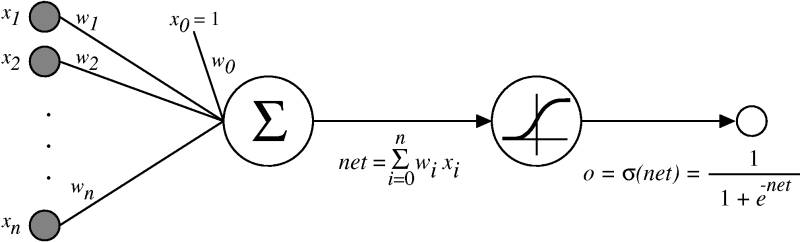
\includegraphics[width=\linewidth]{img/sigmoid-neuron.png}
	\caption{Model neuronu}
	\label{img:model-neuronu}
\end{figure}

W~pierwszej fazie działania neuronu sumowane są wartości na~wejściach neuronu pomnożone przez~odpowiadające
im~wagi. W~drugiej fazie dla~otrzymanej sumy obliczana jest wartość funkcji sigmoidalnej
$f(x)=\frac{1}{1+e^{-x}}$, która stanowi wartość wyjściową neuronu.

Innym często stosowanym neuronem jest neuron o progowej funkcji aktywacji, tzn.~dla~wartości powyżej pewnego
progu przyjmuje wartość 1, a~dla~pozostałych wartości przyjmuje 0 (lub -1). Wyjścia jednostek tego typu
zazwyczaj są~jednocześnie wyjściami całej sieci neuronowej i~nie~są przesyłane na~wejścia innych neuronów.

\subsection{Funkcje aktywacji}
W~neuronach wykorzystywane są bardzo różne funkcje aktywacji (\cite{activation-functions}). Każda z~nich ma swoje
zalety i~wady. W~niniejszej podsekcji przedstawiono i~omówiono wybrane funkcje.

\subsubsection{Funkcja liniowa}
Najprostsza z~możliwych funkcji aktywacji. Dokonuje liniowego przekształcenia na~wartości wejściowej
(rys.~\ref{rys:f-liniowa}). Jest rzadko stosowana do~zadań klasyfikacji w~sieciach neuronowych, gdyż~sieć składająca
się~z~neuronów o~liniowej~funkcji aktywacji nie~może modelować nieliniowych funkcji. Wynika to~z~tego, że~rezultatem
złożenia funkcji liniowych jest również funkcja liniowa. Stąd zastosowania neuronów o~takiej funkcji aktywacji są
mocno ograniczone.

\begin{minipage}[t]{\textwidth}
\begin{equation}
f(x)=x
\end{equation}
\begin{figure}[H]
    \centering
    \begin{tikzpicture}
        \begin{axis}[
            scale only axis, % The height and width argument only apply to the actual axis
            height=5cm,
            width=0.9\textwidth,
            xtick={-1,1},
            axis x line=center, axis y line=center,
            xlabel=$x$,
            ylabel=$f(x)$
            ]
            \addplot [
                domain=-1.1:1.1,
                color=red
            ]{x};
        \end{axis}
    \end{tikzpicture}
    \caption{Funkcja liniowa}
    \label{rys:f-liniowa}

\end{figure}
\end{minipage}

\subsubsection{Funkcja progowa}
Funkcja nieliniowa, a~więc nadająca się~do~zadań klasyfikacji. Posiada jednak wadę przeszkadzającą w~uczeniu sieci
z~wykorzystaniem metod gradientowych: nie~ma~ciągłej pierwszej pochodniej. Funkcja została przedstawiona na~rysunku
\ref{rys:f.progowa}.

\begin{minipage}[t]{\textwidth}
\begin{equation}
	f(x) =
	\begin{cases}
	0 & x<0, \\
	1 & \textrm{w p.p.}
	\end{cases}
\end{equation}

\begin{figure}[H]
    \centering
    \begin{tikzpicture}
        \begin{axis}[
            scale only axis, % The height and width argument only apply to the actual axis
            height=5cm,
            width=0.9\textwidth,
            xmin=-3,xmax=3,
            ymin=-0.5,ymax=1.5,
            axis x line=center,
            axis y line=center,
            xtick={-3,3},
            ytick={-0.25, 0 , 0.5, 1},
            xlabel=$x$,
            ylabel=$f(x)$]
            \addplot[red, samples=1000] {(x>=0)};
        \end{axis}
    \end{tikzpicture}
    \caption{Funkcja progowa}
    \label{rys:f.progowa}
\end{figure}
\end{minipage}

\subsubsection{Funkcja sigmoidalna}
Również jest to~funkcja nieliniowa. W~przeciwieństwie do~funkcji poprzedniej jest gładka. Jednakże również nie~jest
pozbawiona wad~--~przyczynia się~ona~do~powstawania problemu zanikającego gradientu (\cite{vanishing-gradient}),
co~wynika z~tego, że~dla~wysokich wartości wejściowych tej funkcji aktywacji jej gradient jest bliski zera (patrz
rys.~\ref{rys:f.sigmoidalna}).

\begin{minipage}[t]{\textwidth}
\begin{equation}
	f(x) = \frac{1}{1+e^{-x}}
\end{equation}

\begin{figure}[H]
    \centering
    \begin{tikzpicture}
        \begin{axis}[
            scale only axis, % The height and width argument only apply to the actual axis
            height=5cm,
            width=0.9\textwidth,
            xmin=-10,xmax=10,
            ymin=-0.5,ymax=1.5,
            axis x line=center,
            axis y line=center,
            xtick={-10,10},
            ytick={-0.25, 0 , 0.5, 1},
            xlabel=$x$,
            ylabel=$f(x)$]
            \addplot[red, domain=-10:10] {1/(1+e^(-x))};
        \end{axis}
    \end{tikzpicture}
    \caption{Funkcja sigmoidalna}
    \label{rys:f.sigmoidalna}
\end{figure}
\end{minipage}

\subsubsection{Poprawiona jednostka liniowa (\textit{ang. Rectified Linear Unit, ReLU})}
Funkcja ta,~zwana również funkcją rampy (\textit{ang.~ramp function}) jest jedną z~najczęściej wykorzystywanych funkcji
aktywacji w~nowoczesnych rozbudowanych sieciach neuronowych. Jej wady, to~brak pochodnej dla~wartości 0~oraz potencjalny
problem zanikającego gradientu~--~gdy~wagi wejść neuronu przyjmą takie wartości, że~do~funkcji aktywacji będą trafiać
wartości ujemne, wówczas neuron będzie ciągle generować wartość wyjściową równą zero (patrz rys.~\ref{rys:f.rampy}).
Wówczas potocznie mówi się~o~,,śmierci'' neuronu.

\begin{minipage}[t]{\textwidth}
\begin{equation}
	f(x) = max(0,x)
\end{equation}
\begin{figure}[H]
    \centering
    \begin{tikzpicture}
        \begin{axis}[
            scale only axis, % The height and width argument only apply to the actual axis
            height=5cm,
            width=0.9\textwidth,
            xmin=-5,xmax=5,
            ymin=-0.5, ymax=5.5,
            axis x line=center,
            axis y line=center,
            xtick={-4, -2, 0, 2, 4},
            ytick={0, 2, 4},
            xlabel=$x$,
            ylabel=$f(x)$]
            \addplot[red, domain=-5:5] {max(0,x)};
        \end{axis}
    \end{tikzpicture}
    \caption{Funkcja rampy (tzw.~ReLU)}
    \label{rys:f.rampy}
\end{figure}
\end{minipage}

\subsubsection{Funkcja softplus}
Jest to~wartiant funkcji ReLU, który jest jej ,,wygładzoną'' wersją. Posiada ciągłą pierwszą pochodną będącą funkcją
sigmoidalną (\ref{rys:f.sigmoidalna}). Funkcję softplus przedstawiono na~rys.~\ref{rys:f.softplus}.

\begin{minipage}[t]{\textwidth}
\begin{equation}
	f(x) = ln(1 + e^x)  \hspace{1cm} f'(x) = \frac{1}{1 + e^{-x}}
\end{equation}
\begin{figure}[H]
    \centering
    \begin{tikzpicture}
        \begin{axis}[
            scale only axis, % The height and width argument only apply to the actual axis
            height=5cm,
            width=0.9\textwidth,
            xmin=-5,xmax=5,
            ymin=-0.5, ymax=5.5,
            axis x line=center,
            axis y line=center,
            xtick={-4, -2, 0, 2, 4},
            ytick={0, 2, 4},
            xlabel=$x$,
            ylabel=$f(x)$]
            \addplot[red, domain=-5:5] {ln(1 + e^x)};
        \end{axis}
    \end{tikzpicture}
    \caption{Funkcja softplus}
    \label{rys:f.softplus}
\end{figure}
\end{minipage}

\subsubsection{Funkcja softmax}
Funkcja ta~najczęściej stosowana jest w~warstwie wyjściowej sieci. Bywa nazywana \textbf{znormalizowaną funkcją
eksponencjalną}, gdyż~jej wartość to~wartość funkcji eksponencjalnej podzielona przez~sumę wartości wyjściowych innych
neuronów składających się~na~daną warstwę.

Niestety, funkcję softmax ciężko przdstawić na~wykresie, gdyż~jej wartość zależy od~wartości wyjściowych
innych neuronów, przez co dziedzina funkcji jest wielowymiarowa (liczba wymiarów zależy od~liczby neuronów
umieszczonych w~danej warstwie).

\section{Warstwowa sieć neuronowa}
Przy~tworzeniu sztucznej sieci neuronowej ważnym czynnikiem mającym istotny wpływ na~sposób rozwiązania
zadanego problemu, jest dobór odpowiedniego typu sieci. Obecnie najczęściej wykorzystywane są sieci:
\begin{itemize}
  \item jednokierunkowe,
  \item rekurencyjne,
  \item komórkowe.
\end{itemize}

\subsection{Sieć jednokierunkowa}
Jednym z~najczęściej wykorzystywanych typów sieci jest sieć jednokierunkowa. Charakterystyczną cechą takiej
sieci jest brak sprzężeń zwrotnych, tzn. sygnały przesyłane są~od~warstwy wejściowej poprzez warstwy ukryte
aż do~warstwy wyjściowej. Model przykładowej sieci warstwowej przedstawiono poniżej na~rys.~\ref{rys.siec-feed-forward}.

\begin{figure}[H]
	\centering
	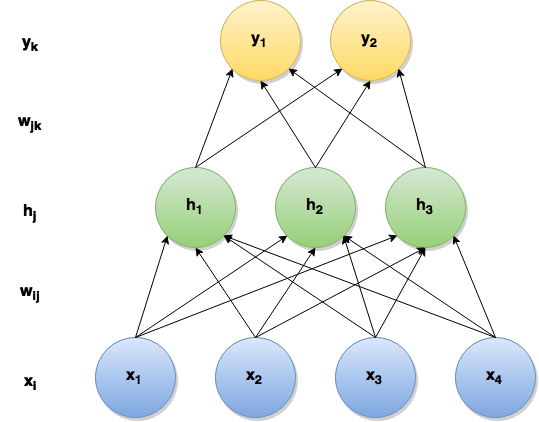
\includegraphics[width=0.9\linewidth]{img/mgr_backprop_net.png}
	\caption{Wielowarstwowa sieć jednokierunkowa}
	\label{rys.siec-feed-forward}
\end{figure}

\subsection{Wsteczna propagacja błędów} \label{ssec:backpropagation}
Wsteczna propagacja błędów jest podstawową metodą uczenia nadzorowanego wielowarstwowych jednokierunkowych
sieci neuronowych. Poprzez uczenie nadzorowane należy rozumieć proces uczenia, w~którym sieć neuronowa
otrzymuje dane wraz z~ich etykietami (spodziewanym wyjściem sieci).

W~pierwszym kroku uczenia należy zdefiniować funkcję straty $Loss(w)$ przyjmującą jako~argument wektor wag
sieci neuronowej. Funkcją tą może być średni błąd kwadratowy, dla danych ciągłych:\\
$$Loss(w)=\frac{1}{2}\sum\limits_{m}(\sigma(w^{T}x^{(m)}) - y^{(m)})^2$$
lub entropia krzyżowa, dla danych binarnych:
$$Loss(w)=-\sum\limits_m(\sigma(w^{T}x^{(m)})\log{y^{(m)}} + (1-\sigma(w^{T}x^{(m)})\log{(1-y^{(m)})})
$$
gdzie:
\begin{minipage}[t]{\textwidth}
\begin{itemize}
  \item w - wagi sieci neuronowej,
  \item m - numer próbki uczącej,
  \item x - wartości wejściowe,
  \item y - spodziewane wartości wyjściowe,
  \item $\sigma$ - funkcja aktywacji.
\end{itemize}
\end{minipage}

Celem uczenia sieci jest minimalizacja funkcji $Loss(w)$. Na~początku należy określić gradient funkcji straty
względem wag sieci (gradient jest taki sam dla obu wymienionych powyżej funkcji).
Następnie można przystąpić do~optymalizacji tej~funkcji wykorzystując metodę gradientu prostego.
Kroki tego algorytmu przedstawiono poniżej:
\begin{enumerate}
  \item zainicjuj losowo wektor wag w,
  \item oblicz gradient funkcji straty,
  \item $w:=w-\alpha \nabla Loss(w)$, $\alpha$ - współczynnik określający długość kroku,
  \item wróć do~kroku 2. jeśli nie~został spełniony warunek stopu.
\end{enumerate}

Zakładając, że~wartość błędu dla~danego przykładu wyraża się~wzorem
$$Error^{(m)}=\sigma(w^{T}x^{(m)})-y^{(m)}$$
gradient funkcji straty ma~wzór:
$$\nabla_{w}Loss=\sum\limits_{m}Error^{(m)}\sigma'(w^{T}x^{(m)})x^{(m)}$$
Ponieważ $\sigma(x)=\frac{1}{1+e^{-x}}$, pochodna funkcji sigmoidalnej wyraża się~wzorem:
$$\sigma'(x)=\sigma(x)(1-\sigma(x))$$

Dla uproszczenia załóżmy, że~w~sieci występuje tylko jedna warstwa ukryta. Wówczas gradient funkcji straty
względem wag połączeń pomiędzy warstwą wyjściową, a~ukrytą:
$$\frac{\partial Loss}{\partial w_{jk}}=\frac{\partial Loss}{\partial in_k}\frac{\partial
in_k}{\partial w_{jk}}= \delta_k \frac{\partial (\sum\limits_j w_{jk}h_j)}{\partial w_{jk}} = \delta_k h_j$$
Poprzez $in_k$ oznaczono wektor wejść trafiających do~funkcji aktywacji poszczególnych neuronów warstwy
wyjściowej.

Gradient funkcjii straty względem wag połączeń pomiędzy warstwą wejściową a~ukrytą:
$$ \frac{\partial Loss}{\partial w_{ij}}=\frac{\partial Loss}{\partial in_j}\frac{\partial in_j}{\partial
w_{ij}} = \delta_j \frac{\partial (\sum\limits_j w_{ij}x_i)}{\partial w_{ij}} = \delta_j x_i $$

$$ \delta_k = \frac{\partial}{\partial in_k}(\sum\limits_k \frac{1}{2}
[\sigma(in_k)-y_k]^2)=[\sigma(\in_k)-y_k]\sigma'(in_k)$$

$$ \delta_j = \sum\limits_k\frac{\partial Loss}{\partial in_k}\frac{\partial in_k}{\partial
in_j}=\sum\limits_k \delta_k \cdot \frac{\partial}{\partial in_j}(\sum\limits_j w_{jk}\sigma(in_j))=[\sum\limits_k \delta_k
w_{jk}]\sigma'(in_j)$$

Jak widać w~ostatnim wzorze: wykorzystujemy gradient obliczony dla~warstwy wyjściowej
do~obliczenia gradientu dla~poprzedniej warstwy. Przy~większej liczbie warstw w~sieci gradienty
dla~kolejnych warstw są~obliczane analogicznie (na~podstawie wartości obliczanych w~następnych warstwach).
Stąd właśnie metoda ta nosi nazwę wstecznej propagacji błędów.


\section{Ogólna koncepcja głębokiego uczenia}
Sama koncepcja głębokiego uczenia nie jest szczególnie nowa. Sieci
wielowarstwowe uczone za pomocą wstecznej propagacji błędów istnieją
już~od~ponad 40 lat. Sieciom tym~towarzyszy jednak poważna wada: przy~wielu
warstwach w~sieci, wagi wyjść początkowych warstw są aktualizowane w~bardzo
nieznacznym stopniu (na ogół: im~większa odległość warstwy od~wyjścia,
tym~mniejsze korekcje wag). W~literaturze problem ten nazywany jest problemem
zanikającego gradientu (\textit{ang. vanishing gradient problem}). Z~tego
powodu do~efektywnego uczenia metodą wstecznej propagacji błędów konieczne jest
stosowanie niewielkiej liczby warstw (w~praktyce stosowano przeważnie
do~czterech warstw). Choć teoretycznie zastosowanie dwóch warstw
wystarcza do~aproksymacji dowolnej funkcji, to~jednak może wymagać bardzo dużej
liczby neuronów w~warstwie ukrytej (w~niektórych problemach liczba neuronów w~warstwie ukrytej może rosnąć
wykładniczo względem rozmiaru danych wejściowych).

Rozwiązaniem problemu zanikającego gradientu jest zastosowanie dodatkowego
etapu: tzw.~uczenia wstępnego (\textit{ang.~pre-training}). W~tym~etapie
optymalizowaną funkcją nie~jest funkcja błędu (jak~w~przypadku metody wstecznej
propagacji błędu), ale~funkcja prawdopodobieństwa wystąpienia danych p(v),
gdzie v stanowi dane wejściowe sieci. Celem, do~którego dąży etap uczenia
wstępnego jest takie uformowanie funkcji p(v), by~dla~danych podobnych do~tych obserwowanych w~zbiorze
uczącym wartość funkcji prawdopodobieństwa była jak największa, natomiast dla pozostałych danych:
jak~najmniejsza.

Opisana metoda uczenia wstępnego zakłada, że~po~kolei uczona jest każda
z~warstw (nie~wszystkie na~raz), zaczynając od~warstwy wejściowej, kończąc
na~wyjściowej. W~jednej iteracji algorytmu uczone są wagi tylko jednej z~warstw.
W~pierwszym kroku algorytmu uczona jest pierwsza warstwa ukryta i~efektem
uczenia powinno być wyodrębnienie takich cech danych, które odróżniają
je~od~danych losowych. W~drugim etapie kolejna warstwa jest uczona w~taki
sposób, by~była w~stanie odróżnić kombinację cech występujących w~danych
od~losowej kombinacji cech itd. Istotną różnicą tej metody w~stosunku do~metody
wstecznej propagacji błędu jest uczenie tylko jednej warstwy na~raz
(po~nauczeniu danej warstwy jej wagi nie~są już modyfikowane w~etapie uczenia
wstępnego). Tak nauczona sieć, choć jeszcze nie~nadaje się~do~przeprowadzania
klasyfikacji, to~dobrze modeluje charakter danych, tzn.~właściwości danych,
które często pojawiają się~w~zestawie uczącym. Na~rys.~\ref{rys:hierarchical-learning} przedstawiono wizualizację
hierarchicznego uczenia się~sieci neuronowej (pierwsza warstwa rozpoznająca najprostsze cechy, kolejne rozpoznające
coraz to~bardziej złożone kombinacje cech).

Po~etapie uczenia wstępnego następuje tzw. dostrajanie sieci
(\textit{ang.~fine-tuning}). W~tym etapie dodawana jest warstwa wyjściowa sieci.
Następnie cała sieć jest uczona danymi etykietowanymi (uczenie nadzorowane)
metodą wstecznej propagacji błędu. Dzięki zastosowaniu uczenia wstępnego
sztuczna sieć neuronowa znacznie lepiej generalizuje funkcję, którą ma~modelować
(tzn.~jest znacznie mniej podatna na~tzw.~overfitting, czyli zbytnie dopasowanie modelu do~danych).
Ponadto, do~dostrajania jest potrzebna znacznie mniejsza ilość danych niż do~pierwszego etapu. Zatem
do~uczenia sieci wystarczy, by~tylko niewielka część danych uczących była
etykietowana.

\begin{figure}[H]
	\centering
	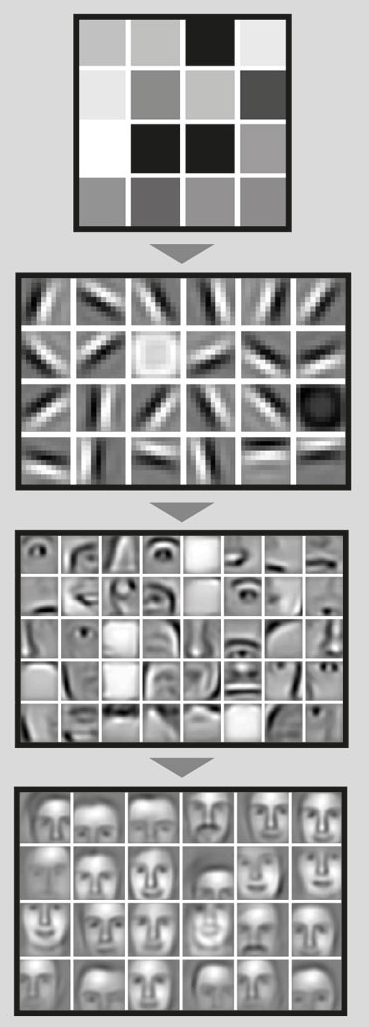
\includegraphics[width=0.45\linewidth]{img/hierarchical-learning_cropped.jpg}
	\caption{Wizualizacja działania neuronów w~kolejnych warswach sieci neuronowej rozpoznającej twarze.
	Źródło:~Stanford University}
	\label{rys:hierarchical-learning}
\end{figure}

\section{Modelowanie funkcji prawdopodobieństwa}
Cechą wspólną wszystkich mechanizmów głębokiego uczenia badanych w~ramach tej~pracy magisterskiej jest
wykorzystanie etapu uczenia wstępnego, którego celem jest odpowiednie zamodelowanie
funkcji rozkładu prawdopodobieństwa, tzn.~osiągnięcie takiego rozkładu prawdopodobieństwa p(v),
że~danym~wejściowym v, które są podobne do~danych uczących, będą odpowiadały wysokie wartości
funkcji prawdopodobieństwa, natomiast pozostałym danym (w~szczególności danym losowym) będzie odpowiadało
niskie prawdopodobieństwo.

Do modelowania funkcji prawdopodobieństwa można wykorzystać wiele mechanizmów. W~tej~pracy omówione zostaną
jedynie poniższe mechanizmy:
\begin{itemize}
    \item \textbf{autoenkoder} (\textit{ang.~autoencoder}),
    \item \textbf{ograniczona maszyna Boltzmanna} (\textit{ang.~Restricted Boltzmann Machine}).
\end{itemize}

\subsection{Autoenkoder}
Autoenkoder \cite{Autoencoder} to~sieć neuronowa, która składa się z~trzech warstw:
\begin{itemize}
	\item warstwy wejściowej,
	\item warstwy ukrytej,
	\item warstwy wyjściowej.
\end{itemize}

Dodatkowo liczba neuronów w~warstwie wyjściowej jest równa liczbie neuronów w~warstwie wejściowej.
Celem uczenia autoenkodera jest osiągnięcie stanu, w~którym wartości na~jego wyjściu są równe
wartościom wejściowym. Wówczas sieć realizuje przekształcenie tożsamościowe.

Przykładową strukturę autoenkodera zaprezentowano na~rys.~\ref{rys:autoenkoder}.
\begin{figure}[H]
	\centering
	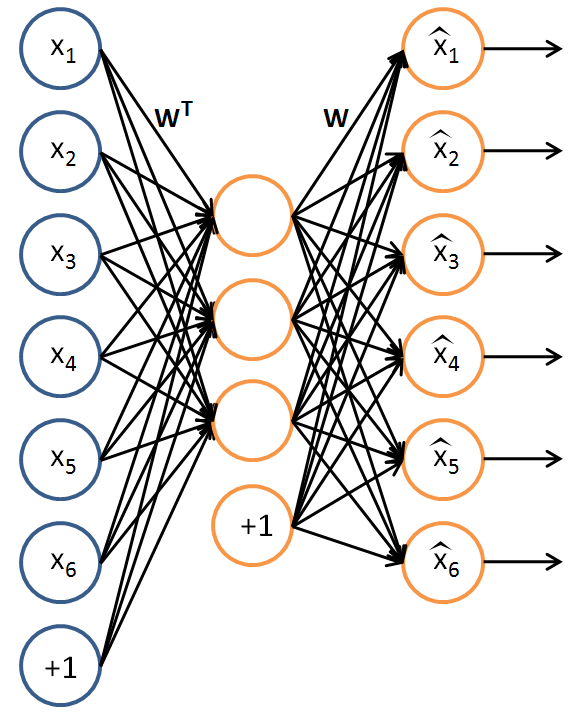
\includegraphics[width=0.75\linewidth]{img/autoencoder.png}
	\caption{Autoenkoder}
	\label{rys:autoenkoder}
\end{figure}

\subsubsection{Zastosowania}
Zazwyczaj w~warstwie ukrytej takiej sieci umieszcza się~mniej neuronów niż~w~dwóch pozostałych warstwach.
Neurony tej warstwy w~procesie uczenia zaczynają wykrywać różne często pojawiające się powiązania
wśród wartości wejściowych (np.~mogą zauważyć, że gdy pierwsza z~wartości jest równa jeden,
wówczas trzecia i czwarta są równe zero itp.).
Pozwala to~na~kompresję danych.

Innym zastosowaniem mechanizmu autoenkodera jest korekcja danych. Wówczas w~warstwie ukrytej
może być więcej neuronów niż w~warstwie wejściowej/wyjściowej. Tak nauczona sieć, po~otrzymaniu na~wejściu
wektora wejściowego zawierającego pewne błędy w~danych (np.~szumy), potrafi dokonać korekty danych,
a dane poprawione pojawią się~na~wyjściu sieci.

W~ogólności warstwa wejściowa oraz warstwa ukryta autoenkodera tworzą razem mechanizm kodujący, a~warstwa ukryta wraz
z~warstwą wyjściową tworzą mechanizm dekodujący.

\subsubsection{Funkcja kosztu}
Dla danych ciągłych ($x\in\mathbb{R}$) jako funkcję kosztu typowo stosuje się~średni kwadrat błędu:
\begin{equation*}
\frac{1}{2N}\sum\limits_{i=1}^{s_1}(x-\hat{x})^2
\end{equation*}
gdzie $N$ to~liczba klasyfikowanych przykładów, $s_1$ to~długość wektora wejściowego (jak~również wyjściowego),
$x$ to~wektor wartości wejściowych, a~$\hat{x}$ to~wektor wartości wyjściowych. Suma dzielona jest przez $2N$ zamiast
$N$ w~celu~wygodniejszego liczenia pochodnej w~procesie uczenia. Zabieg ten ma charakter czysto techniczny.

\subsubsection{Regularyzacja rozrzutu}
W~autoenkoderze staramy się~zapewnić, by~średnia wartość na~wyjściu każdego neuronu warstwy ukrytej
(średnia liczona po~przykładach uczących) była bliska pewnej z~góry przyjętej wartości zwanej \textbf{parametrem
rozrzutu} (\textit{ang.~sparsity parameter}). Zwykle parametr ten przyjmuje niewielkie wartości (np. 0,05). Dzięki temu
dla~większości danych wejściowych niewiele neuronów warstwy ukrytej będzie ,,aktywowanych'', a~więc każdy neuron będzie
rozpoznawał jedną wybraną zależność pomiędzy danymi i~będzie stwierdzał czy~w~danym wektorze wejściowym jest ona obecna
(wartość na~wyjściu neuronu równa 1) czy też nie (wartość na~wyjściu neuronu równa 0). W~celu osiągnięcia odpowiedniego
rozrzutu funkcja celu musi przyjmować odpowienio wyższe wartości, gdy wartość średnia dla wzbudenia neuronu warstwy
ukrytej jest różna od~zadanego parametru rozrzutu. Założony cel można osiągnąć poprzez zastosowanie funkcji kosztu
w~postaci dywergencji Kullbacka-Leiblera:
\begin{equation*}
\sum\limits_{j=1}^{s_2}KL(\rho||\hat{\rho_j}) = \sum\limits_{j=1}^{s_2}\rho \log\frac{\rho}{\hat{\rho_j}} +
(1-\rho)\log\frac{1-\rho}{1-\hat{\rho_j}}
\end{equation*}
gdzie $s_2$ to~liczba neuronów w~warstwie ukrytej, j to~numer neuronu w~warstwie ukrytej, $\rho$~to~parametr rozrzutu,
a~$\hat{\rho_j}$ to~średnia wartość na~wyjściu j-tego neuronu wartstwy ukrytej.

Po~uwzględnieniu regularyzacji, funkcja kosztu przyjmie postać:
\begin{equation*}
J(W,b)=\frac{1}{2N}\sum\limits_{i=1}^{s_1}(x-\hat{x})^2 + \beta\sum\limits_{j=1}^{s_2}KL(\rho||\hat{\rho_j})
\end{equation*}
gdzie $W$ i $b$, to~odpowiednio wagi sieci i~przesunięcie (\textit{ang.~bias}).

\subsubsection{Uczenie}
Do~uczenia sieci wykorzystywana jest metoda wstecznej propagacji błędów (opisana we~wcześniejszej części pracy),
stąd proces zmiany wag w~sieci zaczyna się~od~warstwy wyjściowej. Zdefiniujmy różnicę pomiędzy wartościami wyjściowymi
a wejściowymi jako $\delta_i^{(3)}$, gdzie $i$ jest numerem neuronu w~warstwie wejściowej (lub wyjściowej, bo~neurony
wyjściowe odpowiadają, neuronom wejściowym).
Wagi warstwy wyjściowej aktualizujemy wg wzoru \ref{eqn:wagi_autenc}:
\begin{equation}
    \begin{split}
    W'_i &= W_i + \alpha\delta^{(2)}_i \\
    \delta_i^{(2)} &= \left( \left( \sum\limits_{j=1}^{s_{2}} W^{(2)}_{ji} \delta^{(3)}_j \right)
    + \beta \left( - \frac{\rho}{\hat\rho_i} + \frac{1-\rho}{1-\hat\rho_i} \right) \right) f'(z^{(2)}_i)
    \end{split}
    \label{eqn:wagi_autenc}
\end{equation}
gdzie $f'$ to~pochodna funkcji aktywacji używanej w~neuronach, a~$z^{(2)}_i$, to~wartości całkowitego wzbudzenia
(\textit{ang.~preactivation}) neuronów warstwy ukrytej (wartości, które trafiają do~funkcji aktywacji tych neuronów).

Wagi wastwy ukrytej odpowiadają transponowanej macierzy wag warstwy wyjściowej. Jest tak~dlatego, że~jak~wcześniej
wspomniano, warstwa wyjściowa odpowiada za~operację odwrotną do~operacji wykonywanej przez~warstwę ukrytą (odpowiednio:
dekodowanie i kodowanie).

\subsection{Ograniczona maszyna Boltzmanna}
Ograniczona maszyna Boltzmanna jest sztuczną siecią neuronową składającą się~z~dwóch warstw neuronów:
\begin{itemize}
  \item warstwy neuronów widocznych,
  \item warstwy neuronow ukrytych.
\end{itemize}

Tytułowe ograniczenie mechanizmu polega na~tym, że~neurony należące do~tej~samej warstwy nie~są ze~sobą połączone,
czyli bezpośrednio nie~wymieniają żadnych informacji (w~przeciwieństwie do~oryginalnego mechanizmu: maszyny Boltzmanna).
Zadaniem ograniczonej maszyny Boltzmanna, podobnie jak~autoenkodera, jest rekonstrukcja danych wejściowych.

Mechanizm zaprezentowano na~rysunku \ref{rys:restricted-boltzmann-machine}. Górna warstwa,
to~warstwa neuronów ukrytych. Co~ciekawe, dolna warstwa~--warstwa widoczna~--~to~zarówno warstwa wejściowa,
jak~i~wyjściowa. Wynika to~z~natury mechanizmu, który po~przyjęciu pewnych danych wejściowych przekształca je,
a~wartości przekształcone przedstawiane są na~wyjściach neuronów wejściowych.

\begin{figure}[H]
	\centering
	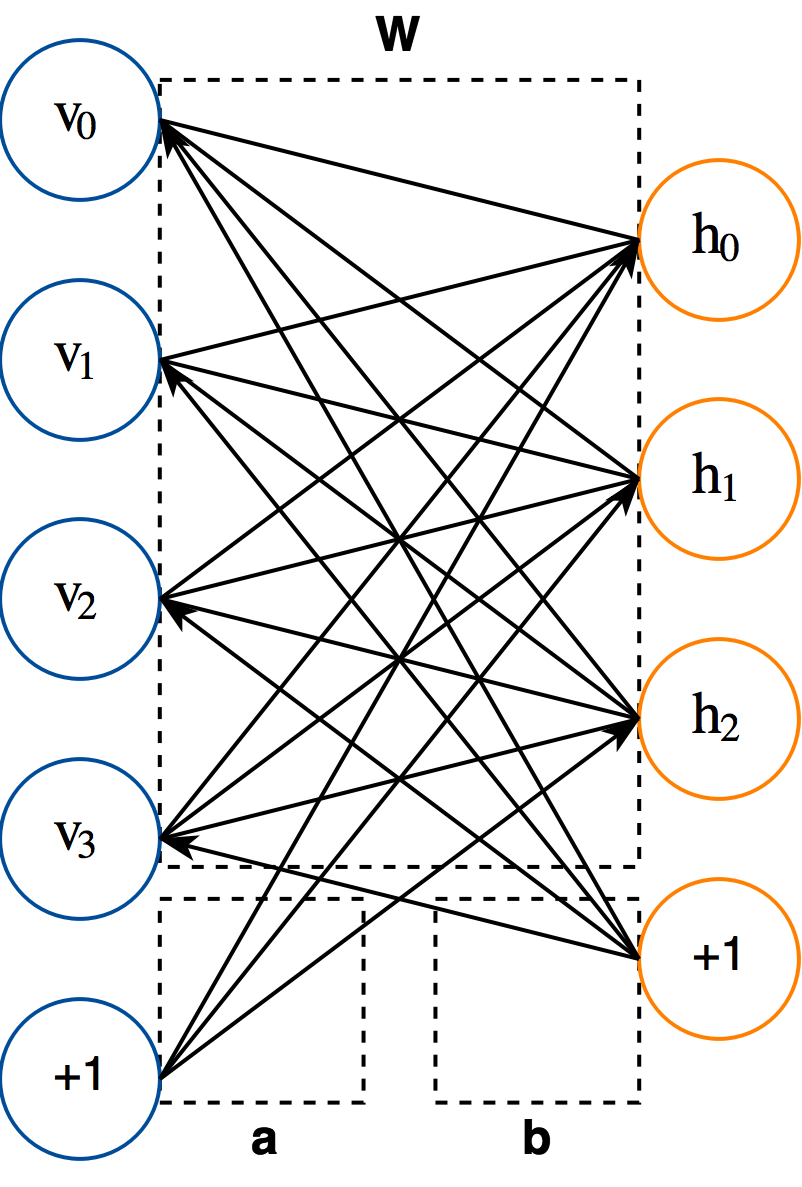
\includegraphics[width=0.65\linewidth]{img/RBM.png}
	\caption{Ograniczona maszyna Boltzmanna. Na~rysunku: lewa warstwa to~warstwa widoczna, a~warstwa z~prawej strony
	to~warstwa widoczna, pełniąca rolę zarówno warstwy wejściowej, jak~i~wyjściowej. $a$~i~$b$ to~przesunięcia
(\textit{ang.~bias}), a~$W$~to~wagi połączeń pomiędzy neuronami widocznymi i~ukrytymi.}
	\label{rys:restricted-boltzmann-machine}
\end{figure}

Cechą charakterystyczną omawianego mechanizmu jest jego umiejętność do~wyodrębniania cech danych wejściowych
(\textit{ang. feature extraction}). Przykładowo: ograniczona maszyna Boltzmanna, którą uczono obrazkami, będzie
wykrywać charakterystyczne łuki czy krawędzie.

Dzięki tej właściwości mechanizm może być wykorzystywany m.in. do~korekcji danych.

\subsubsection{Prawdopodobieństwo stanów sieci}
W~ograniczonej maszynie Boltzmanna każdy stan sieci (tzn. zestaw wartości wyjść poszczególnych neuronów)
ma~określone prawdopodobieństwo zadane wzorem:

$p(v,h)=\frac{1}{Z}e^{-E(v,h)}$, gdzie:
\begin{itemize}
  \item v to~wektor wyjść neuronów widocznych,
  \item h to~wektor wyjść neuronów ukrytych,
  \item Z to~czynnik normalizujący (tzw.~funkcja partycji),
  \item $E(v,h)=-a^{T}v-b^{T}h-v^{T}Wh$,
  \item W to~macierz wag sieci (wagi połączeń między neuronami),
  \item a, b to~odpowiednio wektor przesunięć (ang.~bias) dla~neuronów warstwy widocznej i~neuronów warstwy ukrytej.
\end{itemize}

\subsubsection{Inferencja}
Ze~względu na~to, że~neurony nie~łączą się~ze~sobą w~obrębie tej~samej warstwy, wartość na~wyjściu każdego
neuronu w~danej warstwie można uzyskać wyłącznie na~podstawie wartości wyjść neuronów drugiej warstwy.
Prawdopodobieństwa wzbudzeń neuronów można efektywnie obliczyć korzystając ze~wzorów:
\begin{equation}
    \begin{split}
        p(h_{j}=1|v)&=\sigma(b_{j}+\sum\limits_{i=1}^{m}w_{i,j}v_{i}) \\
        p(v_{i}=1|h)&=\sigma(a_{i}+\sum\limits_{j=1}^{n}w_{i,j}h_{j})
    \end{split}
	\label{eqn:rbm_inference}
\end{equation}
gdzie: $\sigma$ to~funkcja aktywacji, $i$ oraz $j$ to~numery kolejnych neuronów (odpowiednio: wejściowych i~ukrytych).


\subsubsection{Uczenie}
Celem uczenia sieci jest znalezienie takich parametrów a, b i W, że~wartość funkcji prawdopodobieństwa p(v)
dla~danych obserwowanych będzie wysoka, a~dla~pozostałych danych niska. W~praktyce zamiast maksymalizować
funkcję prawdopodobieństwa p(v), minimalizuje się funkcję średniego ujemnego logarytmu prawdopodobieństwa,
gdzie średnia jest liczona po~wszystkich $T$ przykładach ze~zbioru uczącego:
\begin{equation*}
\frac{1}{T}\sum\limits_{t}-\log{p(v^{(t)})}
\end{equation*}
gdzie $t$ to~numer przykładu uczącego.

Do~minimalizacji funkcji metodami gradientowymi konieczne jest obliczenie pochodnej po~parametrach sieci ($\theta$)
dla tej funkcji:
$$\frac{\partial-\log{p(v^{(t)})}}{\partial{\theta}}=\mathbb{E}_h[\frac{\partial{E(v^{(t)},h)}}{\partial{\theta}}\mid{v^{(t)}}]-\mathbb{E}_{v,h}[\frac{\partial{E(v,h)}}{\partial{\theta}}]$$

Pierwszy ze~składników sumy występującej w~powyższym wzorze to~tzw. składnik pozytywny. Drugi składnik
to~tzw.~składnik negatywny. Pierwszy z~nich odpowiada zwiększaniu wartości funkcji prawdopodobieństwa
dla~obserwowanych danych, a~drugi zmniejsza prawdopodobieństwo danych nieobserwowanych. Drugi składnik jest
skomplikowany obliczeniowo, gdyż występuje w~nim iteracja po~wszystkich możliwych stanach sieci, których
liczba rośnie wykładniczo względem liczby neuronów w~sieci. Z~tego powodu dokonuje się estymacji. Jedną
z~wykorzystywanych metod jest tzw.~próbkowanie Gibbsa.

\textbf{Próbkowanie Gibbsa} pozwala wyeliminować problem obliczania wartości oczekiwanej dla~wszystkich
możliwych stanów sieci. Zamiast tego wartość ta~jest estymowana za~pomocą algorytmu, którego kroki
przedstawiono poniżej.

Próbkowanie Gibbsa (algorytm):
\begin{enumerate}
  \item Oblicz wartości wyjściowe dla~każdego neuronu z~warstwy ukrytej na~podstawie danych wejściowych
  (korzystając ze~wzorów \ref{eqn:rbm_inference}).
  \item Oblicz wartości wyjściowe dla~każdego neuronu z~warstwy wejściowej na~podstawie obliczonych wartości
  wyjściowych neuronów ukrytych (korzystając z~wzorów \ref{eqn:rbm_inference}).
\end{enumerate}

Kroki 1 i 2 mogą być powtarzane wielokrotnie, choć w~praktyce okazuje się, że wystarczy jeden
przebieg algorytmu. Otrzymane w~punkcie drugim ,,odtworzone'' wartości wejścia oznaczane są~jako $\tilde{v}$.

\paragraph{Aktualizacja parametrów sieci}
Parametry (wagi) sieci aktualizowane są według następujących wzorów:
\begin{itemize}
  \item $W_t=W_{t-1}+\alpha(h(v^{(t)})v^{(t)T}-h(\tilde{v})\tilde{v}^{T})$
  \item $b_t=b_{t-1}+\alpha(h(v^{(t)})-h(\tilde{v}))$
  \item $a_t=a_{t-1}+\alpha(v^{(t)})-\tilde{v})$
\end{itemize}
\vspace{1cm}

Przez $h(v)$ oznaczono wartości wyjściowe neuronów ukrytych obliczone na~podstawie wartości wyjściowych
neuronów wejściowych.

\chapter{Splotowe sieci neuronowe}
Splotowe sieci neuronowe są wielowarstwowymi sieciami jednokierunkowymi. Charakteryzuje je~możliwość
wykrywania wzorców występujących w~różnych fragmentach przetwarzanego obrazu (np. rozpoznawanie oka
w~dowolnym fragmencie obrazka). Zasada ich~działania była inspirowana neurobiologią, a~mianowicie analizowano
sposób przetwarzania informacji przez~ośrodek wzrokowy kota.

\section{Filtry splotowe}
Splot dyskrentny jako pojęcie matematyczne jest zdefiniowany w~następujący sposób:
$$ f\ast g[n]\defeq \sum\limits_{m=-\infty}^{\infty}f[m]g[n-m] = \sum\limits_{m=-\infty}^{\infty}f[n-m]g[m]$$

W~cyfrowym przetwarzaniu obrazów filtry splotowe znajdują bardzo szerokie zastosowanie, gdyż w~zależności
od~dobranej maski filtra, osiągane są różne rezultaty. Przykładowe filtry splotowe:
\begin{itemize}
  \item filtr Gaussa (wygładzanie),
  \item filtr Laplace'a (wyostrzanie).
\end{itemize}
Maski dla~wymienionych filtrów są~z~góry ustalone i~nie~ulegają zmianie w~czasie działania algorytmu. Splotowa
sieć neuronowa zamiast wykorzystywać z~góry określone maski, ,,uczy się ich'', a~więc stara się~tak dobrać
ich~wartości, aby~jak~najlepiej rozpoznawać wyznaczone obiekty na~obrazach. Poszczególnym wartościom
w~masce filtra odpowiadają wagi splotowej sieci neuronowej. 

\subsection{Padding}
Przy~stosowaniu filtrów splotowych pojawia się problem: jaką wartość powinny otrzymać piksele obrazka
znajdujące się na jego krawędzi. Jest on~rozwiązywany poprzez rozszerzanie obrazka o~dodatkowe piksele
na~jego krawędziach. Można tego dokonać m.in. poprzez:
\begin{itemize}
  \item rozszerzenie obrazka o~czarne piksele (tzw.~\textit{zero-padding}),
  \item rozszerzenie obrazka odbicia lustrzane pikseli przy krawędziach.
\end{itemize}

\section{Inferencja}
W~trakcie działania sieci na~obrazie dokonywanie jest filtrowanie splotowe (przy wykorzystaniu różnych
filtrów). Po~takim filtrowaniu otrzymywane jest $n\cdot m$ obrazów, nazywanych mapami cech
(\textit{ang.~features maps}), gdzie n~-~liczba początkowych obrazów (tzw.~kanałów wejściowych), m~-~liczba
użytych filtrów.

Po~dokonaniu filtrowania splotowego obrazy są skalowane na~mniejsze (tzw.~faza pooling/subsampling) i~znów
stosowane są~filtry splotowe. Oba kroki (filtrowanie i~skalowanie) są~powtarzane wielokrotnie
(zależy od~liczby warstw sieci), aż~do~osiągnięcia odpowiednio wyskokopoziomowych cech. Liczba warstw oraz
liczba filtrów splotowych wykorzystanych w każdej z~nich jest ustalana podczas fazy projektowania sieci.

\begin{figure}[H]
	\centering
	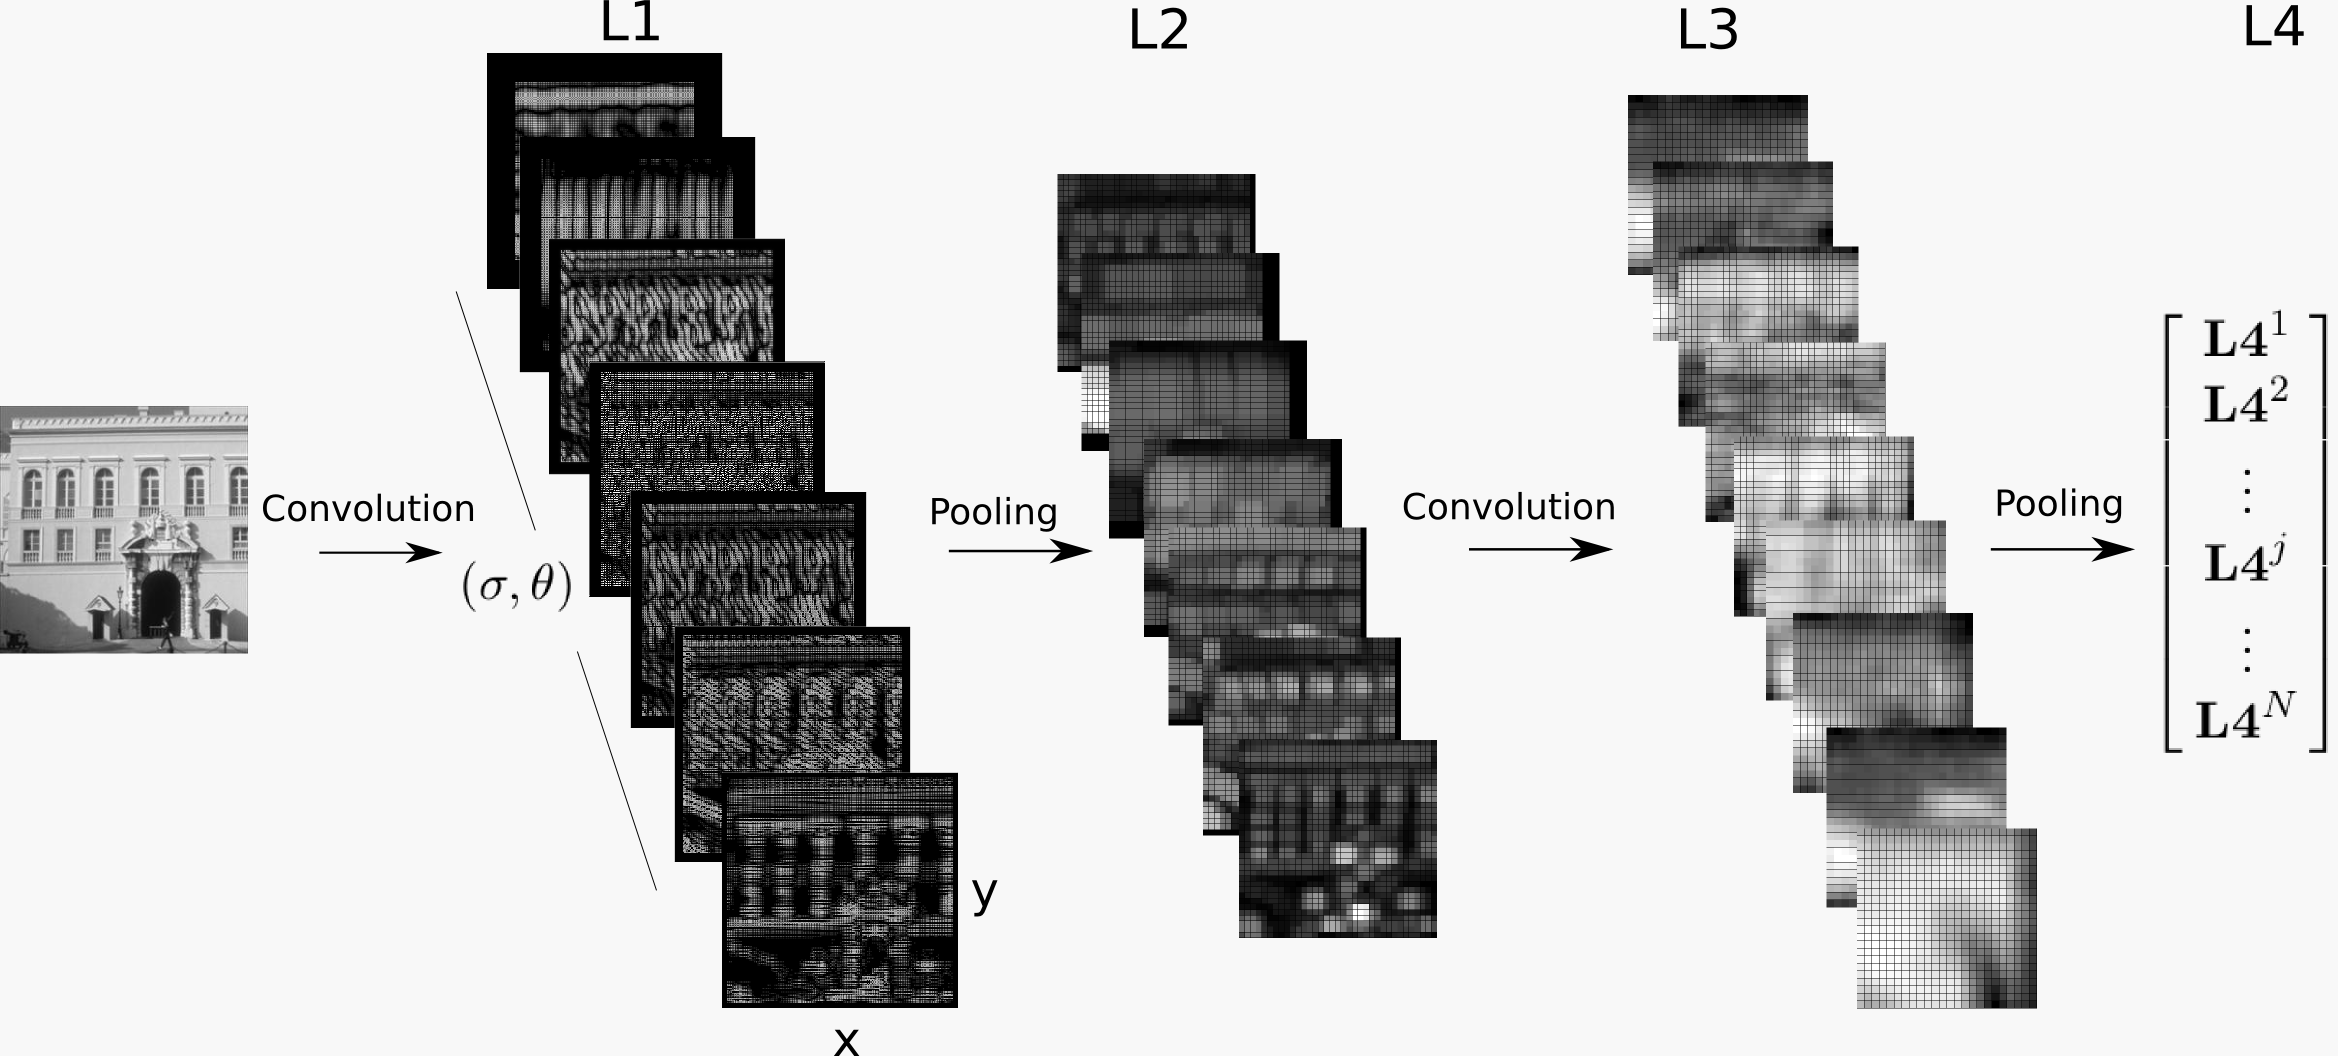
\includegraphics[width=\linewidth]{img/convnet.png}
\end{figure}

Ostatnią warstwą sieci (zazwyczaj otrzymującą dużo bardzo małych obrazów) jest warstwa zawierająca neurony
sigmoidalne. Każdy neuron warstwy wyjściowej jest połączony ze~wszystkimi wartościami otrzymanymi na~wyjściu
poprzedniej warstwy.

\subsection{Skalowanie}
Po zastosowaniu n różnych filtrów splotowych w~danej warstwie na m różnych mapach cech, powstaje $n\cdot m$
kolejnych map cech. Stąd ilość przetwarzanych danych szybko rośnie wraz z~dokładaniem kolejnych warstw
w~sieci. Aby temu przeciwdziałać stosuje się skalowanie obrazów pomiędzy warstwami dokonującymi splotu.
Najczęściej obraz skalowany jest poprzez:
\begin{enumerate}
  \item podzielenie obrazka na~nienachodzące na~siebie kwadratowe obszary,
  \item wybranie z~każdego obszaru piksela o~największej wartości (tzw.~\textit{max-pooling}). 
\end{enumerate}

Alternatywnie, w drugim kroku algorytmu można wybrać medianę wartości pikseli\\
(\textit{ang.~mean-pooling}) lub~wartość średnią (\textit{average-pooling}).

\subsection{Możliwe ulepszenia sieci}
TODO rectification(prostowanie/rektyfikacja???), local contrast normalization(lokalna normalizacja kontrastu),
dropout

\section{Uczenie metodą wstecznej propagacji}
Typową metodą uczenia sieci jest wsteczna propagacja błędów. W~tym celu należy obliczyć gradient funkcji
straty względem wag sieci (wartości masek filtrów splotowych) dla~warstw:
\begin{itemize}
  \item wyjściowych,
  \item skalujących,
  \item splotowych.
\end{itemize}
Obliczanie gradientu funkcji straty dla~warstw zawierających neurony sigmoidalne zostało omówione
w~sekcji (\ref{ssec:backpropagation}), stąd wyjaśnienia wymaga jedynie obliczanie gradientów dla~warstw skalujących i~splotowych.

\subsection{Obliczanie gradientu dla~warstw skalujących}
Znając gradient funkcji straty $\nabla_{y_{ijk}}l$ z~warstwy kolejnej, można w prosty sposób policzyć gradient
w~stosunku do~wejścia warstwy dla~której jest on liczony. W~przypadku, gdy~warstwa wykorzystywała algorytm
\textit{max-pooling}, gradient względem wejść warstwy przyjme wartość:
\begin{itemize}
  \item $\nabla_{x_ijk}l = \nabla_{y_{ijk}}l$, dla~pikseli, które miały maksymalną wartość w~obszarze, 
  \item $\nabla_{x_ijk}l = 0$, dla~pozostałych pikseli.
\end{itemize}

\subsection{Obliczanie gradientu dla~warstw splotowych}
Przy~wstecznej propagacji błędów z~warstwy kolejnej otrzymujemy gradient błędu względem wyjścia
aktualnej warstwy $\nabla_{y_j}l$. Do~aktualizacji wag sieci konieczne jest policzenie gradientu funkcji
straty wzlgędem wag tej warstwy.
$$ \frac{\partial E}{\partial w_{ab}} 
= \sum\limits_{i=0}^{N-m}\sum\limits_{j=0}^{N-m}\frac{\partial E}{\partial x_{ij}^l}\frac{\partial
x_{ij}^l}{\partial w_{ab}}
= \sum\limits_{i=0}^{N-m}\sum\limits_{j=0}^{N-m}\frac{\partial E}{\partial x_{ij}^l}y^{l-1}_{(i+a)(j+b)}$$
gdzie:
\begin{itemize}
  \item $N\times N$ - rozmiar mapy cech,
  \item $m\times m$ - rozmiar filtra,
  \item $x_{ij}^l$ - wartość wejścia neuronu o~wsp. (i,j) w~warstwie l,
  \item $w_{ab}$ - wartość w~masce filtra znajdująca się~na~pozycji (a,b).
\end{itemize}

Następnie należy policzyć tzw.~delty ($\frac{\partial E}{\partial x_{ij}^l}$):
$$\frac{\partial E}{\partial x_{ij}^l} = \frac{\partial E}{\partial y_{ij}^l}\frac{\partial y_{ij}^l}{\partial
x_{ij}^l} =
\frac{\partial E}{\partial y_{ij}^l}\frac{\partial}{\partial x_{ij}^l}(\sigma(x_{ij}^l))
= \frac{\partial E}{\partial y_{ij}^l}\sigma'(x_{ij}^l)
$$

Na~koniec należy policzyć gradient funkcji błędu względem wyjść warstwy poprzedniej (po~to, by~przekazać
go~do~poprzedniej warstwy):
$$ \frac{\partial E}{\partial y_{ij}^{l-1}} =
\sum\limits_{a=0}^{m-1}\sum\limits_{b=0}^{m-1} \frac{\partial E}{\partial x^l_{(i-a)(j-b)}}
\frac{\partial x^l_{(i-a)(j-b)}}{\partial y_{ij}^{l-1}} =
\sum\limits_{a=0}^{m-1}\sum\limits_{b=0}^{m-1} \frac{\partial E}{\partial x^l_{(i-a)(j-b)}}w_{ab}$$

Należy zwrócić uwagę na~dwie rzeczy: po~piersze na~to, że~podczas obliczania gradientów również wykonywany
jest splot jednak na~obrazku o~,,odwróconych'' wierszach i~kolumnach. Dodatkowo, by~móc dokonywać splotu
na~krawędziach map cech, należy zastosować \textit{zero-padding}.

\subsection{Uczenie wstępne}
W~celu lepszego zainicjowania wag sieci należy przeprowadzić uczenie wstępne. W~tym~etapie sieć zamiast uczyć
się rozpoznawania obiektów, ma~za~zadanie nauczyć się~charakteru danych wejściowych (ma~zauważać
charakterystyczne cechy, podobieństwa obiektów it.p.). Do~uczenia wstępnego wykorzystuje się~mechanizmy
uczenia nienadzorowanego, takie jak:
\begin{itemize}
  \item autoenkoder,
  \item RBM (Restricted Boltzmann Machine).
\end{itemize}

Uczenie wstępne przebiega w~następujący sposób:
\begin{enumerate}
  \item wyodrębnienie losowych fragmentów obrazka (tzw.~łatki),
  \item uczenie mechanizmu uczenia nienadzorowanego (np.~RBM),
  \item zainicjowanie wag uczonej warstwy wagami z~tego~mechanizmu,
  \item policzenie map cech dla~łatek,
  \item wykonanie kroków 1-3 dla~uzyskanych map~cech (uczenie wstępne kolejnej warstwy).
\end{enumerate}

\chapter{Opis środowiska}
W celu uniknięcia konieczności zajmowania się niskopoziomowymi problemami, takimi jak:
\begin{itemize}
    \item zrównoleglanie obliczeń wektorowych,
    \item wykonywanie obliczeń na~karcie graficznej,
    \item liczenie gradientów operacji wykonywanych przez sieć neuronową (takich jak~sploty, normalizacje, aktywacje),
    \item wczytywanie danych,
    \item itp.
\end{itemize}
postanowiono skorzystać z~jednej~z~dostępnych bibliotek, która zajmuje się~owymi zagadnieniami. Pozwala to~na~skupienie
się~na~architekturze sieci oraz na odpowiednim doborze operacji mających na~celu zapewnienie jak~najlepszej
klasyfikacji.

\section{Wybrana biblioteka}
Do~realizacji badań wykonywanych w~ramach niniejszej pracy magisterskiej wykorzystano bibliotekę
\textbf{Tensorflow} firmy Google.

W~rozdziale opisano podstawowe zagadnienia dotyczące wybranego narzędzia. Wiedza ta~pozwoli na~zrozumienie
informacji o~architekturze sieci przedstawianych w~dalszych częściach pracy.

\section{Graf operacji}
Tworzenie sztucznej sieci neuronowowej przy~użyciu wymienionej powyżej biblioteki, można podzielić na~dwa etapy:
\begin{enumerate}
    \item zdefiniowanie grafu operacji,
    \item wykonanie wybranych operacji z~grafu.
\end{enumerate}

Graf operacji definiuje w~jaki sposób dane wejściowe mają być przetwarzane po to, by osiągnąć rezultat na wyjściu.
Każda operacja może przyjmować pewne dane wejściowe. Dane wejściowe mogą być zarówno danymi wczytanymi z~dysku
czy~z~klawiatury. Najczęściej jednak są one~wynikami innych operacji. W~ten sposób operacje tworzą wzajemne zależności,
gdzie wyjście jednej z~nich jest jednocześnie wejściem innej. Operacje mogą być ze sobą grupowane poprzez tworzenie
tzw.~zakresów (\textit{ang.~scope}). Przykładowy graf przedstawiono na rysunku \ref{img:tf-smpl-grf}.

\begin{figure}[H]
	\centering
	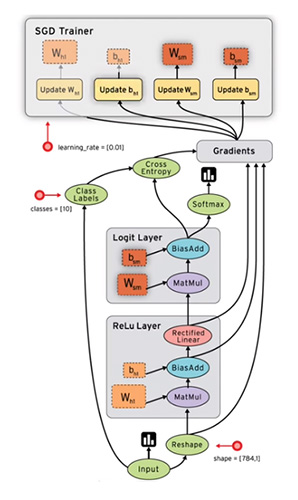
\includegraphics[width=0.5\linewidth]{img/tf-sample-graph.jpg}
	\caption{Przykładowy graf operacji}
	\label{img:tf-smpl-grf}
\end{figure}

\subsection{Konstrukcja grafu}
W pierwszym etapie tworzenia sieci neuronowej należy zdefiniować graf operacji. W~następnym kroku można wykonać
wybrane operacje, a~silnik Tensorflow sam wykona wszystkie akcje wymagane do~poprawnego obliczenia ich rezultatu.

Podczas konstrukcji grafu zamiast konkretnych danych wykorzystywane są dane symboliczne (np.~,,zmienna~x'',
,,dana~C''). Dopiero później, w etapie wykonania operacji, za~niektóre z~owych danych podstawiane
są~odpowiednie wartości (podczas wykonywania operacji do~silnika Tensorflow podawany jest tzw.~kontekst będący
słownikiem odwzorowującym wybrane dane symboliczne na realne wartości).

\pythonexternal{code/graph_creation.py}

\subsection{Wykonanie operacji}
Dwoma naistotniejszymi operacjami wykonywanymi podczas konstrukcji sieci neuronowej będą:
\begin{itemize}
    \item operacja uczenia,
    \item operacja klasyfikacji.
\end{itemize}

Mając już skonstruowany graf operacji, można wykonać dowolną operację zdefiniowaną w~grafie (np.~operację klasyfikacji).

\pythonexternal{code/op_execution.py}

\chapter{Podsumowanie}
W ciągu ostatnich 10 lat dzięki znacznemu wzrostowi mocy obliczeniowej, szczególnie dzięki rozwojowi takich technologii
jak~Nvidia CUDA (\cite{nvidia-cuda}), istotnie wzrosło zainteresowanie sztucznymi sieciami neuronowymi. Znalazły
one~praktyczne zastosowanie w~problemach takich jak:
\begin{itemize}
    \item rozpoznawanie mowy,
    \item rozpoznawanie obrazów,
    \item generowanie sygnałów dźwiękowych,
    \item generowanie danych graficznych (np.~pisma ręcznego),
    \item przetwarzanie języka naturalnego.
\end{itemize}

Między innymi dużym zainteresowaniem cieszą się~mechanizmy służące do~rozpoznawania obrazów takie jak~splotowe sieci
neuronowe. Przetwarzanie obrazów jest ważnym zagadnieniem na~drodze do~stworzenia tzw.~sztucznej inteligencji ogólnego
przeznaczenia (ang.~general purpose artificial intelligence, \cite{strong-AI}). Prace nad~stworzeniem takiego mechanizmu
trwają. Zagadnienie to~jest badane m.in. przez~firmę Google w~ramach projektu DeepMind. Mechanizm rozwijany
przez~przedsiębiorstwo z~Mountain View wykorzystuje uczenie ze~wzmoznieniem wraz ze~splotowymi sieciami neuronowymi.
Stąd, można powiedzieć, że~prace nad~splotowymi sieciami neuronowymi zbliżają ludzkość do~zbudowania uniwersalnego
mechanizmu potrafiącego rozwiązywać zagadnienia z różnych dziedzin, podobnie jak~człowiek.

Rozpoznawanie obrazów pełni znaczącą rolę nawet u~większości zwierząt, o~czym może świadczyć to,~że~ośrodek wzrokowy
u~ssaków jest jednym z~najbardziej złożonych. Przypuszczać można, iż~wynika to~z~tego, że~najwięcej informacji
z~otaczającego świata można pozyskiwać z~sygnałów optycznych. O~tym jak~istotne (a~jednocześnie skomplikowane) jest
to~zagadnienie może świadczyć fakt, iż~prawie połowa kory nowej u~naczelnych odpowiada za~przetwarzanie sygnałów
wzrokowych (\cite{primate-cerebral-cortex}).

Obecnie splotowe sieci neuronowe są~przedmiotem wielu badań oraz znajdują zastosowanie w~wielu problemach. Istnieją
nawet portale~ogłaszające konkursy, w~których dla~twórców najlepszych mechanizmów przewidziane są~zwykle wysokie nagrody
pieniężne (np. Kaggle, \cite{kaggle-competitions}). Splotowe sieci neuronowe zdobywają większość nagród w~konkursach
dotyczących rozpoznawania obrazów.

W~niniejszej pracy magisterskiej badana sieć miała dość prostą architekturę, dzięki czemu jej uczenie nie~wymagało
zastosowania wysokich mocy obliczeniowych oraz nie~pochłaniało dużych ilości czasu. Dzięki temu możliwe było
przeprowadzenia wielu badań w~stosunkowo krótkim czasie (zwykle pojedyncze badanie nie~trwało dużej niż~4~dni).
Opisana sieć może być wykorzystana w~przyszłości do~badań nad~nowymi metodami poprawiającymi zarówno dokładność
klasyfikacji (np.~dropout, warstwy typu batch normalization), jak~i~jej szybkość (np.~zmodyfikowane wersje
zaprezentowanej architektury, inne modele neuronów, różne rozmiary wsadu z~przykładami w~procesie uczenia).

W~zastosowniach profesjonalnych (np.~prace wygrywające konkursy na~stronie Kaggle) zwykle stosowane są~bardzo złożone
architektury, do~uczenia których wykorzystywane są~komputery z~wieloma (np.~czterema) kartami graficzymi. Sam proces
uczenia takich mechanizmów zwykle liczony jest w~tygodniach lub~miesiącach (a~nie pojedycznych dniach, jak~w~przypadku
sieci opisywanej w~ramach niniejszej pracy magisterskiej). Jednakże owa~sieć może być rozbudowana o~dodatkowe warstwy
i~dodatkowe mechanizmy. Ponadto została ona~zaimplementowana w~taki sposób, by~obliczenia wykonywane w~procesie uczenia
mogły wykorzystywać wiele kart graficznych.

Rozbudowana wersja sieci, wykorzystująca 15~warstw i~uczona przy~użyciu czterech kart graficznych, zostanie zgłoszona
do~konkursu ogłoszonego przez The Nature Conservacy (\cite{nature-conservacy}). Problem opublikowany na~stronie Kaggle
dotyczy rozpoznawania na~zdjęciach różnych gatunków ryb (m.in.~różnych gatunków tuńczyków i~rekinów) złowionych
przez~łodzie rybackie na~Zachodnim i~Środkowym Pacyfiku.
\chapter{Badania}
\section{Wykorzystywana miara jakości klasyfikatora}
Podstawowymi miarami stosowanymi w~ocenie jakości sieci neuronowych są:
\begin{itemize}
    \item dokładność (\textit{ang.~accuracy}),
    \item średnia precyzja (\textit{ang.~average precision}).
\end{itemize}

\paragraph{Dokładność} wskazuje jaka część przykładów ze~zbioru ewaluacyjnego została sklasyfikowana poprawnie.
\begin{equation*}
    ACC = \frac{CP}{T}
\end{equation*}
gdzie $CP$ to~liczba poprawnie sklasyfikowanych przykładów, a~$T$ to~całkowita liczba przykładów.

Jeśli wśród przykładów istnieje spora nadreprezentacja przykładów jednej klasy wówczas wskaźnik ten~może być
niemiarodajny. Przykładowo: klasyfikator mający stwierdzać płeć wśród studentów Wydziału Elektroniki i~Technik
Informacyjnych Politechniki Warszawskiej mógłby wsakzywać dla~każdej osoby płeć męską, a~jego dokładność byłaby
dość wysoka. Dlatego w~takich przypadkach badając jakość sieci należy posłużyć się~również dodatkowymi miarami.

\paragraph{Precyzja} to~miara, która liczona jest dla~każdej z~klas z~osobna i~wyraża ile~przykładów sklasyfikowanych
 jako należące do~danej~klasy faktycznie należy do~tej klasy (przykładowo: jaka część obrazów sklasyfikowanych jako
 obraz z~psem faktycznie jest obrazem przedstawiającym to~zwierzę). W~ocenie jakości sieci neuronowych rozpoznających
 więcej niż~dwie klasy stosuje się~uśrednioną precyzję, tj.~średnią z~precyzji uzyskanych dla~każdej z~klas.
 \begin{equation*}
    PPV = \frac{TP}{TP+FP}
\end{equation*}
gdzie $TP$ to~prawidłowo rozpoznane przykłady danej klasy, a~$FP$ to~przykłady niepoprawnie sklasyfikowane jako
 należące do~tej klasy.

\section{Środowisko sprzętowe}
Badania zostały wykonane z wykorzystaniem następującego zestawu komputerowego:
\begin{itemize}
    \item \textbf{procesor}~--~Intel Core i7-4771 3,5Ghz (8 rdzeni),
    \item \textbf{płyta główna}~--~MSI~B85M-G43,
    \item \textbf{karta graficzna}~--~MSI GeForce GTX 780 Ti,
    \item \textbf{pamięć RAM}~--~2 x GoodRam 8GB 1600 MHz.
\end{itemize}

\section{Architektura sieci neuronowej}
Podczas tworzenia splotowej sieci neuronowej, należy dobrać wiele hiperparametrów takich jak:
\begin{itemize}
    \item liczba warstw splotowych,
    \item liczba jąder stosowanych do~wykonywania splotów w~każdej z~warstw splotowych,
    \item rozkład warstw typu max-pooling (\ref{sec:inferencja}),
    \item rozkład warstw normalizujących (\ref{sssec:normalizacja_odpowiedzi}),
    \item współczynnik uczenia (\ref{ssec:backpropagation}).
\end{itemize}

Ogólne zasady dotyczące pierwszych dwóch z~wymienionych punktów zostały opisane w~artykule
,,Rethinking the Inception Architecture for Computer Vision''(\cite{RIACV}). Posiłkując się~przytoczoną pracą można
wymienić kilka wskazówek przydatnych przy~ustalaniu hiperparametrów sieci:
\begin{itemize}
    \item unikanie zbyt małej liczby neuronów w~warstwach, w~sczególności w~warstwach początkowych. Warto zastosować
          kilkukrotność/kilkunastokrotność spodziewanej liczby klas, które ma~rozpoznawać sieć
          (w~przypadku CIFAR-10 jest to~10 klas). Warstwy końcowe mogą zawierać mniejszą liczbę neuronów, niż warstwy
          poprzednie.
    \item zmniejszenie rozmiaru danych wejściowych poprzez zastosowanie metod, takich jak:
          \begin{itemize}
              \item usunięcie brzegów, gdyż~zwykle zawierają mało istotne dane,
              \item zmniejszenie rozmiaru obrazka poprzez zastosowanie sklaowania.
          \end{itemize}
    \item używanie niewielkich filtrów splotowych (np. 3x3 lub 5x5 zamiast 7x7). Lepsze efekty daje zastosowanie dwóch
          warstw splotowych o~maskach 3x3 niż jednej maski 7x7,
    \item warto zacząć od~2 do~5 warstw splotowych (tyle samo warstw skalujących i~normalizujących), następnie zwiększać
          liczbę masek używanych w~warstwach splotowych na~przemian ze~zwiększaniem liczby warstw.
\end{itemize}

\subsection{Architektura badanej sieci} \label{ssec:architektura-podstawowa}
Badana sieć w~swojej podstawowej wersji bazuje na~architekturze AlexNet przedstawionej w~artykule \cite{AlexNet}.
Po dokonaniu drobnych modyfikacji w~końcowych etapach przetwarzania obrazu, sieć składa się~z~następujących warstw:
\begin{enumerate}
    \item Warstwy splotowej z~64 maskami o rozmiarze 5x5x3 (wysokość x szerokość x liczba objętych kanałów).
          Maska przesuwana jest zawsze o~1~piksel (w~kierunku pionowym lub~poziomym).
    \item Warstwy skalującej typu max-pooling o~wielkości filtra 3x3x1 (wysokość x szerokość x liczba objętych kanałów).
          Filtr jest przesuwany o~2~piksele (w~kierunku pionowym lub~poziomym)
    \item Warstwy normalizującej (normalizacja lokalnej odpowiedzi).
    \item Warstwy splotowej z~64 maskami o rozmiarze 5x5x64 (wysokość~x~szerokość~x~liczba objętych kanałów).
          Maska przesuwana jest zawsze o~1 piksel (niezależnie od~kierunku przesuwania maski).
    \item Warstwy normalizującej (normalizacja lokalnej odpowiedzi).
    \item Warstwy skalującej typu max-pooling o~wielkości filtra 3x3x1 (wysokość~x~szerokość~x~liczba objętych kanałów).
          Filtr jest przesuwany o~2~piksele (w~kierunku pionowym lub~poziomym).
    \item Warstwy w~pełni połączonej (standardowa warstwa w~sieciach neuronowych) z~384 neuronami i~funkcją aktywacji
          typu ReLU.
    \item Warstwy w~pełni połączonej z~192 neuronami i~funkcją aktywacji
          typu ReLU.
    \item Warstwy wyjściowej (również w~pełni połączonej) z~10 neuronami (tyle samo, co~klas do~rozpoznawania).
          Warstwa wyjściowa zawiera funkcję aktywacji typu softmax.
\end{enumerate}

\subsubsection{Przetwarzanie wstępne}
Dane wejściowe przed~tym, jak~trafią do~sieci neuronowej, poddawane są~przetwarzaniu wstępnemu. Sprowadza się~ono
do~przycięcia obrazka, tak~by~jego rozdzielczość wyniosła 24x24 piksele (oryginalna: 32x32 piksele). W~procesie
uczenia obrazek przycinany jest losowo, a~w~przypadku obrazka klasyfikowanego~--~wybierany jest środkowy fragment.
Dodatkowo, jeśli obrazek ma~być wykorzystywany w~procesie uczenia, poddawany jest on~zniekształceniu.

Po~wczytaniu i~przycięciu obrazka (w~przypadku uczenia: również po~zastosowaniu zniekształcenia) każdy z~obrazów jest
normalizowany (niezależnie od~innych). Normalizacja polega na~zapewnieniu, że~subpiksele w~każdym kanale
przyciętego obrazka (czerwonym, zielonym i~niebieskim) mają średnią wartość równą zero i~odchylenie standardowe równe~1.

%\subsubsection{Graf operacji}
%Powyższy opis architektury sieci ilustruje graf operacji (\ref{sec:graf-operacji}).
%\begin{figure}[H]
%	\centering
%	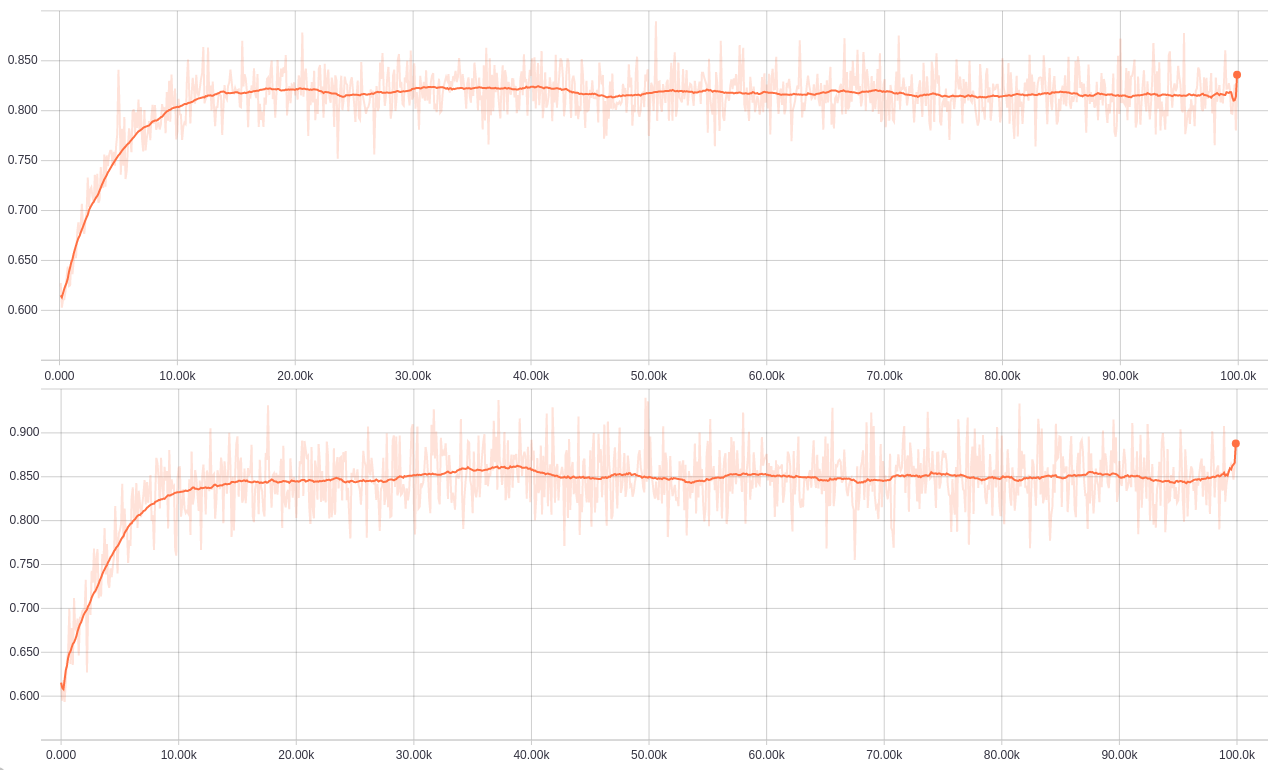
\includegraphics[width=\linewidth]{img/badanie_1.png}
%	\caption{Dokładność na zbiorze walidacyjnym (górny wykres) i uczącym (dolny wykres)}
%	\label{rys:badanie-1}
%\end{figure}
%
%% TODO dodać obrazek przedstawiający graf operacji


\section{Plan badań} \label{sec:plan-badan}
Celem niniejszej pracy magisterskiej jest sprawdzenie jak istotny wpływ na~dokładność klasyfikacji mają 2~czynniki:
\begin{itemize}
    \item regularyzacja typu L2 (\ref{sssec:reg_L2}),
    \item normalizacja lokalnej odpowiedzi (\ref{sssec:normalizacja_odpowiedzi}).
\end{itemize}

W~artykule ,,Practical Recommendations for Gradient-Based Training of Deep Architectures''
(\cite{practical-gradient-based}) skrótowo omówiono problem doboru hiperparametrów sieci. Jednym ze~sposobów
przedstawionych w~opracowaniu jest określenie wartości brzegowych dla~optymalizowanych hiperparametrów,
a~następnie zbadanie przestrzeni między nimi. Po~zbadaniu zachowania sieci dla~tej przestrzeni hiperparametrów, można podjąć
decyzję o~przyjęciu jednego z~zestawów hiperparametrów dla~sieci lub~rozszerzyć pole poszukiwań o~kolejne obszary.

Dla~parametru regularyzacji~L2 (tzw.~\textbf{weight decay}) jako~górne ograniczenie przyjęto początkowo wartość~0.05.
Wybór bazował na~tym, że~w~podobnych sieciach, tj.~przeznaczonych do~identyfikacji obiektów przedstawianych na~obrazkach
z~bazy ImageNet (\cite{imagenet}), wartość tego hiperparametru nie~przekraczała~0.03. Badanie miało sprawdzić
również jak~sieć zachowywałaby~się~bez regularyzacji wag. Stąd jako dolne ograniczenie przyjęto wartość~0.

Dla~parametru decydującego o~wpływie normalizacji lokalnej odpowiedzi (tzw.~parametr $\alpha$) jako ograniczenie górne
przyjęto początkowo wartość~0.001, a~jako ograniczenie dolne wartość~0. Usprawiedliwienie dla~tych decyzji było
takie samo, jak~dla~wyborów dokonanych przy~hiperparametrze regularyzacji~L2.

Dla~każdej pary parametrów sieć była uczona mini-zestawami danych (\textit{ang.~minibatch}), z~których
każdy zawierał 128 przykładów uczących. Po~każdym kroku uczenia pojedynczym mini-zestawem danych, sprawdzano
dokładność sieci na~zbiorze testowym. Po~wykonaniu wszystkich kroków uczenia dla~danej pary hiperparametrów
brano średnią dokładność sieci na~zbiorze testowym ze~100 ostatnich kroków uczenia.

\section{Badanie architektury podstawowej} \label{sec:badanie-1}
W~pierwszym badaniu przeprowadzono proces uczenia sieci o~architekturze opisanej w~sekcji
\ref{ssec:architektura-podstawowa}. Wykorzystano 100 tys. mini-zestawów danych (\textit{ang.~minibatch}).
Wyniki eksperymentu przedstawiono w~tabeli \ref{table:wyniki1}.

\begin{table}[H]
    \centering
    \begin{tabular}{|l|l|l|l|l|l|}
      \hline
                       & $\lambda$ = 0.0005 & $\lambda$ = 0.001 & $\lambda$ = 0.005 & $\lambda$ = 0.01 & $\lambda$ = 0.05 \\
      \hline
      $\alpha=0.00001$ & 0.83 & 0.79 & 0.76 & 0.75 & 0.78 \\
      \hline
      $\alpha=0.00005$ & 0.82 & 0.80 & 0.77 & 0.78 & 0.75 \\
      \hline
      $\alpha=0.0001$  & 0.84 & 0.81 & 0.80 & 0.73 & 0.77 \\
      \hline
      $\alpha=0.0005$  & 0.85 & 0.83 & 0.84 & 0.81 & 0.79 \\
      \hline
      $\alpha=0.001$   & 0.84 & 0.84 & 0.82 & 0.78 & 0.76 \\
      \hline
    \end{tabular}
    \caption{Wpływ regularyzacji L2 ($\lambda$) i~normalizacji lokalnego kontrastu ($\alpha$) na~dokładność klasyfikacji
    sieci neuronowej}
    \label{table:wyniki1}
\end{table}

Całkowity czas badania wyniósł: 40 godzin 10 minut i 58 sekund.

\subsection{Omówienie wyników badań}
Wyniki uzysakne w~badaniu wskazują, że~wzraz ze~wzrostem wpływu regularyzacji~L2 na~sieć neuronową, dokładność
klasyfikacji ulegała pogorszeniu. Jednocześnie najlepsze wyniki osiągane były dla~wartości $\alpha$ w~okolicach 0.0005.

W~przypadku wpływu normalizacji lokalnego kontrastu wyniki są~zgodne z~oczekiwaniami, tj.~dla~odpowiednio dobranych
parametrów normalizacja ta~przynosi poprawę rezultatów. Sprzeczne z~przewidywaniami okazały się~zmiany wartości
dokładności dla~różnych wartości parametru $\lambda$. Spodziewano się, że~regularyzacja zapobiegając przeuczeniu
polepszy dokładność klasyfikacji.

Wytłumaczeniem takiego stanu rzeczy może być brak wystąpienia zjawiska przeuczenia, z~dwóch powodów:
\begin{itemize}
    \item zbyt mała liczba neuronów w~sieci, a~przez~to~niska szansa na~zbytnie dopasowanie się~sieci do~danych
          wejściowych,
    \item zbyt mała liczba iteracji podczas uczenia sieci.
\end{itemize}
Regularyzacja~L2 choć~zapobiega wystąpieniu overfittingu, to~jednak ma~negatywny wpływ na~szybkość uczenia się~sieci,
przez~co~potrzebna jest większa liczba iteracji w~procesie uczenia, aby~osiągnąć zadowalający poziom dokładności.

By~sprawdzić czy~występuje przeuczenie warto posłużyć się~wykresem przedstawiającym dokładność (\textit{ang.~accuracy})
w~zależności od~numeru iteracji uczenia. Na~wykresie \ref{rys:badanie-1} zamieszczono
dokładności liczone na~zbiorze uczącym oraz na~zbiorze walidacyjnym. W~przypadku wystąpienia przeuczenia na~wykresie
powinno się zaobserwować, że~dla~pewnego numeru iteracji pomimo zwiększania się~dokładności na~zbiorze uczącym,
dokładność na~zbiorze walidacyjnym maleje. Na~wykresie \ref{rys:badanie-1} nie~obserwujemy takiej sytuacji.

\begin{figure}[H]
	\centering
	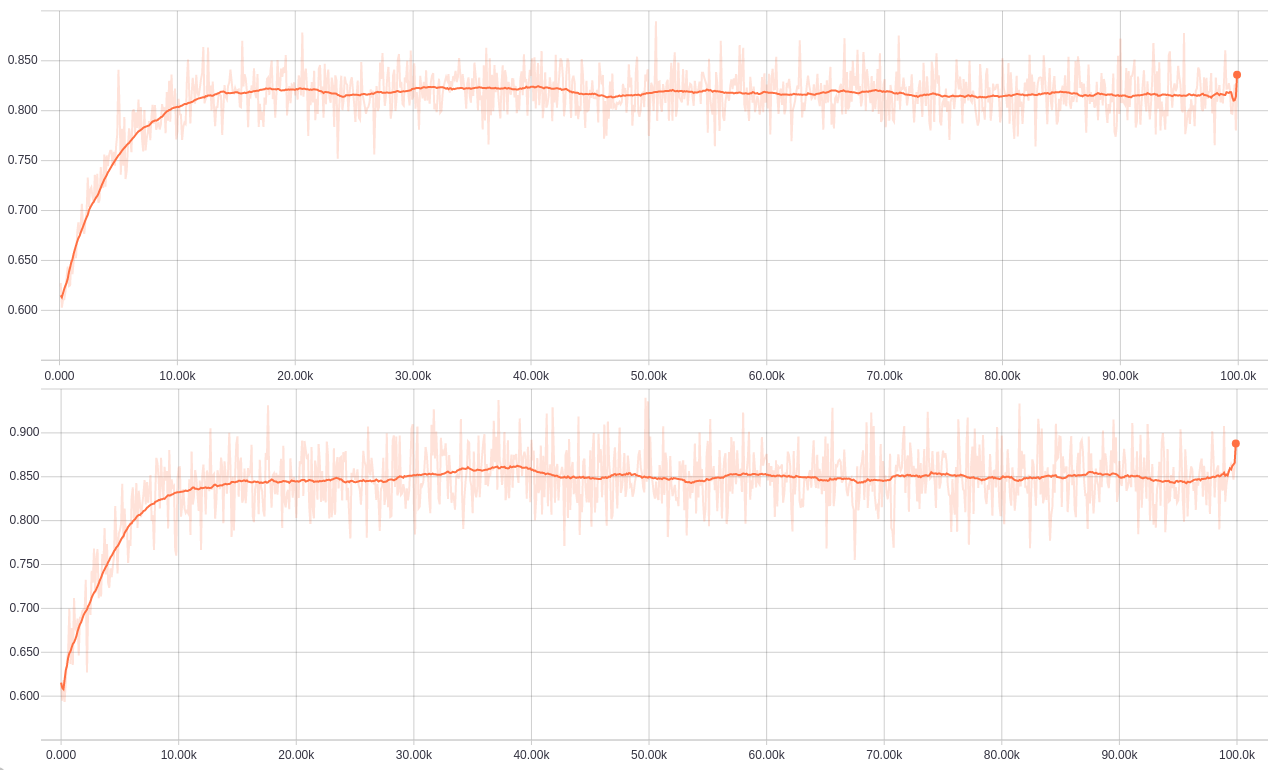
\includegraphics[width=\linewidth]{img/badanie_1.png}
	\caption{Dokładność na zbiorze walidacyjnym (górny wykres) i uczącym (dolny wykres)}
	\label{rys:badanie-1}
\end{figure}

\section{Badanie sieci przy~zwiększonej liczbie iteracji}
W~badaniu nr~2~powtórzono badanie nr~1 (\ref{sec:badanie-1}) ze~zwiększoną liczbą iteracji (do 144000).
Spodziewano się,~że~od~pewnego numeru iteracji będzie obserwowany spadek dokładności na~zbiorze walidacyjnym
przy~jednoczesnym wzroście dokładności na~zbiorze uczącym. Jednakże również nie~udało się~zaobserwować zaistniałej
sytuacji (patrz wykres~\ref{rys:badanie-2}). Prawdopodobnie wynika to~z~tego, że~sieć z~powodu swojej względnie prostej
struktury nie~ma~możliwości przeuczenia się~(zbyt mała liczba neuronów w~stosunku do~liczby przykładów uczących).

\begin{figure}[H]
	\centering
	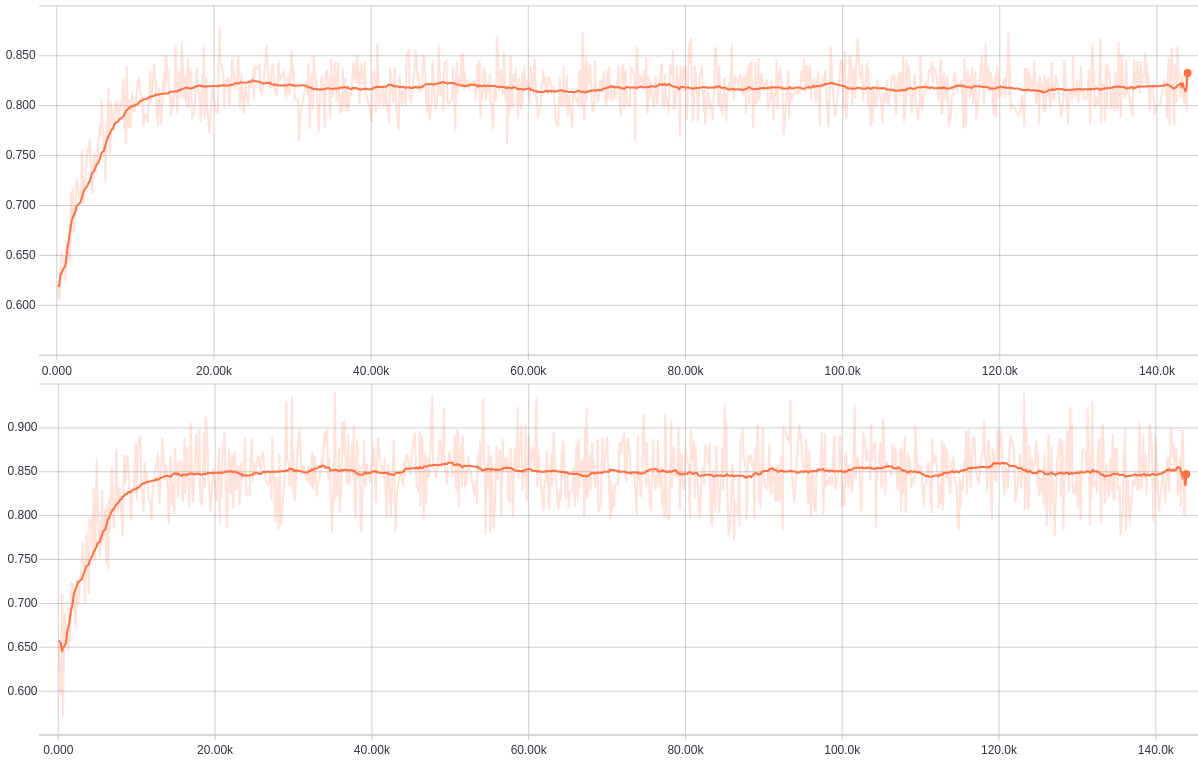
\includegraphics[width=\linewidth]{img/badanie_2.png}
	\caption{Dokładność na zbiorze walidacyjnym (górny wykres) i uczącym (dolny wykres) przy~liczbie iteracji
	         zwiększonej do~144 tysięcy}
	\label{rys:badanie-2}
\end{figure}

Wyniki przedstawiono w~tabeli \ref{table:wyniki2}.

\begin{table}[H]
    \centering
    \begin{tabular}{|l|l|l|l|l|l|}
      \hline
                       & $\lambda$ = 0.0005 & $\lambda$ = 0.001 & $\lambda$ = 0.005 & $\lambda$ = 0.01 & $\lambda$ = 0.05 \\
      \hline
      $\alpha=0.00001$ & 0.90 & 0.89 & 0.87 & 0.83 & 0.82 \\
      \hline
      $\alpha=0.00005$ & 0.91 & 0.88 & 0.85 & 0.83 & 0.84 \\
      \hline
      $\alpha=0.0001$  & 0.90 & 0.88 & 0.88 & 0.87 & 0.87 \\
      \hline
      $\alpha=0.0005$  & 0.92 & 0.92 & 0.89 & 0.87 & 0.86 \\
      \hline
      $\alpha=0.001$   & 0.89 & 0.87 & 0.87 & 0.83 & 0.83 \\
      \hline
    \end{tabular}
    \caption{Wpływ regularyzacji L2 ($\lambda$) i~normalizacji lokalnego kontrastu ($\alpha$) na~dokładność klasyfikacji
    sieci neuronowej przy~liczbie iteracji zwiększonej do~144 tysięcy}
    \label{table:wyniki2}
\end{table}

Całkowity czas badania wyniósł: 64 godziny 17 minut i 23 sekundy.


\section{Badanie na zmniejszonym zbiorze uczącym}
By~sprawdzić jaki wpływ na~dokładność klasyfikacji będzie miała regularyzacja, gdy~problem przeuczenia występuje,
zaprojektowano badanie numer~3, w~którym sześciokrotnie zmniejszono liczbę przykładów w~zbiorze uczącym (przy~zachowaniu
takiego samego rozmiaru zbioru walidacyjnego). Spodziewano się,~że~spowoduje to~wystąpienie zjawiska przeuczenia sieci
(\textit{ang.~overfitting}).

\begin{figure}[H]
	\centering
	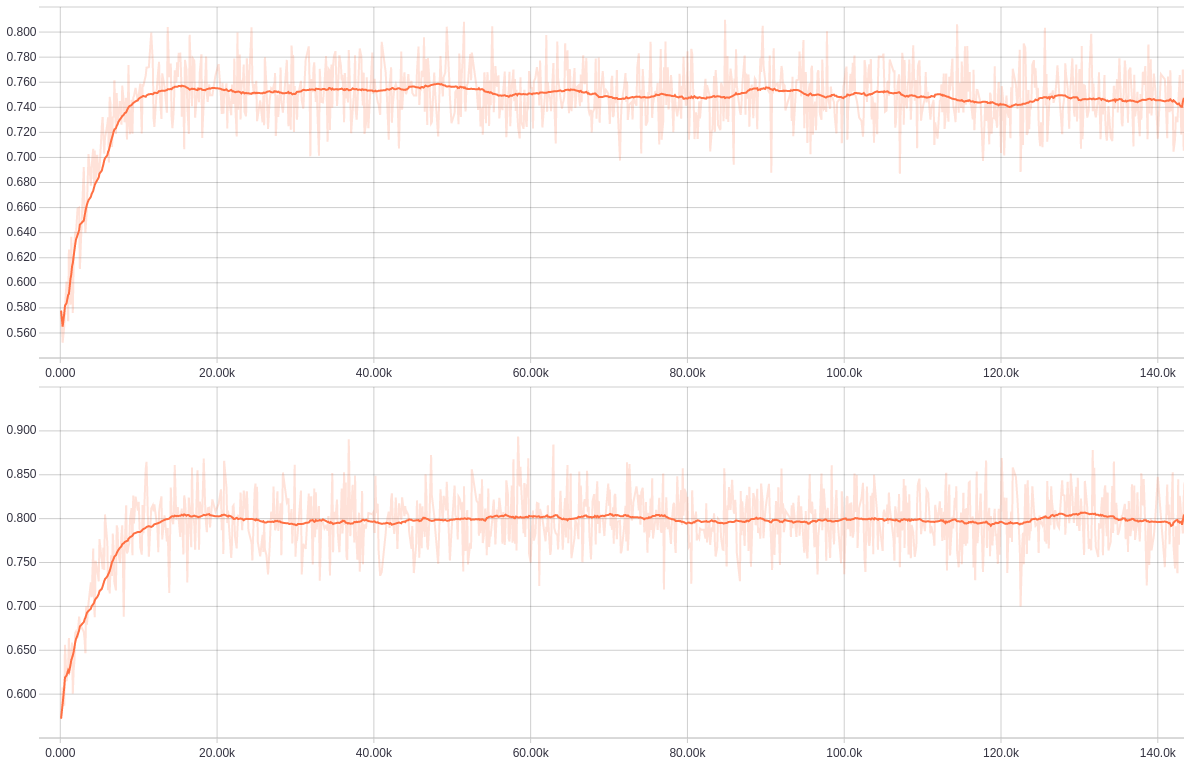
\includegraphics[width=\linewidth]{img/badanie_3.png}
	\caption{Dokładność na zbiorze walidacyjnym (górny wykres) i uczącym (dolny wykres) przy~sześciokrotnie
	         zmniejszonym zbiorze uczącym. Liczba iteracji: 144 tysiące}
	\label{rys:badanie-3}
\end{figure}

Jak~widać na~wykresie \ref{rys:badanie-3} problem przeuczenia zaczyna się~pojawiać w~okolicach iteracji nr~45000.
Stąd należy się~spodziewać, że~regularyzacja zmniejszy występowanie tego niepożądanego zjawiska.

W~tabeli \ref{table:wyniki3} przedstawiono dokładność klasyfikacji dla~różnych kombinacji parametrów normalizacji
i~regularyzacji. Tak~jak~się~spodziewano regularyzacja przy~odpowiednio dobranych metaparametrach
($\alpha=0.0005$ i~$\lambda=0.001$) poprawia jakość klasyfikacji.

\begin{table}[H]
    \centering
    \begin{tabular}{|l|l|l|l|l|l|}
      \hline
                       & $\lambda$ = 0.0005 & $\lambda$ = 0.001 & $\lambda$ = 0.005 & $\lambda$ = 0.01 & $\lambda$ = 0.05 \\
      \hline
      $\alpha=0.00001$ & 0.76 & 0.80 & 0.74 & 0.69 & 0.69 \\
      \hline
      $\alpha=0.00005$ & 0.78 & 0.77 & 0.72 & 0.69 & 0.67 \\
      \hline
      $\alpha=0.0001$  & 0.77 & 0.78 & 0.79 & 0.74 & 0.73 \\
      \hline
      $\alpha=0.0005$  & 0.78 & 0.82 & 0.76 & 0.76 & 0.72 \\
      \hline
      $\alpha=0.001$   & 0.76 & 0.79 & 0.76 & 0.69 & 0.69 \\
      \hline
    \end{tabular}

    \caption{Wpływ regularyzacji L2 ($\lambda$) i~normalizacji lokalnego kontrastu ($\alpha$) na~dokładność klasyfikacji
    sieci neuronowej przy~sześciokrotnie zmniejszonym zbiorze uczącym. Liczba iteracji: 144 tysiące}
    \label{table:wyniki3}
\end{table}

Całkowity czas badania wyniósł: 62 godziny 43 minuty i 27 sekund.

\section{Weryfikacja poprawności działania sieci} \label{sec:weryfikacja-poprawnosci}
Po~dobraniu hiperparametórw sieci warto wykonać badanie pomocnicze mające na celu sprawdzić czy~przy~klasyfikacji
obrazów są~brane pod~uwagę właściwe piksele np.~czy~przy~klasyfikacji obrazu na~którym jest pies, sieć stwierdza,
że~jest to~pies na~podstawie fragmentu obrazu przedstawiającego psa czy~na~podstawie fragmentów nieistotnych.

Przy~poszukiwaniu odpowiedzi na~pytanie: "co~sieć bierze pod~uwagę przy~klasyfikacji obrazów" warto wykorzystać
metody przedstawione w~artykule ,,Visualizing and Understanding Convolutional Networks'' (\cite{understanding-cnn}).
Jedną z~nich~jest metoda, w~której zasłaniane są różne fragmenty klasyfikowanego obrazu i~sprawdzane jest,
jaki ma~to~wpływ na~klasyfikację, a~dokładniej: na~wartość prawdopodobieństwa, że~na~danym obrazku znajduje
się~określony przedmiot.

Przesuwając odpowiednio łatkę (czyli fragment obrazu, który jest ,,zasłaniany'' poprzez zastąpienie go zerami),
uzyskujemy kolejne wartości prawdopodobieństwa, że~na~obrazie znajduje się~przedmiot, który naprawdę się~na~nim
znajduje. Następnie w~utworzonej mapie ciepła na~pozycjach pikseli istotnych z~punktu widzenia klasyfikacji wystąpią
niskie wartości prawdopodobieństwa (co~oznacza, że~po~zasłonięciu tego fragmentu, prawdopodobieństwo poprawnej
klasyfikacji będzie niskie). Natomiast punkty o~wysokiej wartości prawdopodobieństwa odpowiadać będą pikselom
nieistotnym.

\begin{figure}[H]
	\centering
	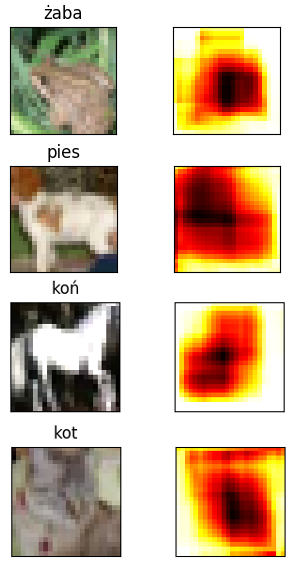
\includegraphics[width=0.75\linewidth]{img/heatmap.png}
	\caption{Mapy ciepła ilustrujące, jak istotne dla klasyfikacji sa dane piksele. Im~piksel ciemniejszy, tym~jest
	ważniejszy. W~pierwszej kolumnie znajdują się~klasyfikowane obrazki, a~w~drugiej odpowiadające im~mapy ciepła}
	\label{rys:badanie-3}
\end{figure}

\section{Wnioski końcowe}
Jak~pokazały przeprowadzone badania zabiegi takie jak~regularyzacja nie~zawsze mają sens. Należy je~stosować wyłącznie
wtedy, kiedy obserwowane jest przeuczenie sieci. W~przeciwnym wypadku zamiast zwiększania jakości klasyfikacji
(wyrażanego jako dokładność), obserwowany jest jej~spadek.

By~sprawdzić czy~przeuczenie sieci występuje warto posłużyć się~wykresem przedstawiającym dokładność sieci na~zbiorze
uczącym i~walidacyjnym mierzoną po~każdej iteracji uczenia. Innym badaniem, które pozwala sprawdzić czy~sieć bierze
pod~uwagę istotne informacje na~zdjęciu jest wykorzystanie map ciepła, w~których im~piksel miał większy wpływ
na~wynik klasyfikacji, tym~,,cieplejszy'' ma kolor (patrz sekcja \ref{sec:weryfikacja-poprawnosci}).

Odpowiednie dobranie metaparametrów sieci nie~jest łatwe. Zwykle dobrze jest bazować na~architekturze innej sieci
wykonującej podobne zadanie (przy~zbiorze \mbox{CIFAR-10} może to~być np.~sieć AlexNet). Następnie w~celu poprawy jakości
klasyfikacji można wykorzystać przeszukiwanie kratowe (\textit{ang.~grid search}), które opisano
w~sekcji~\ref{sec:plan-badan}.

\chapter{Bibliografia}
\begin{itemize}
  \item \href{https://www.youtube.com/playlist?list=PL6Xpj9I5qXYEcOhn7TqghAJ6NAPrNmUBH}{Hugo Larochelle,
  Neural networks class -~Université~de~Sherbrooke:
  http://tinyurl.com/lpkvjm4},
  \item \href{http://deeplearning.net/tutorial/}{DeepLearning.net},
  \item \href{https://www.coursera.org/course/ml}{Stanford University -~Machine Learning:\\
  https://www.coursera.org/course/ml},
  \item \href{http://deeplearning.cs.toronto.edu/i2t}{Image Description Generator: http://deeplearning.cs.toronto.edu/i2t},
  \item \href{http://deeplearning.net/demos/}{Deep Learning - Przykłady: \\
  http://deeplearning.net/demos},
\end{itemize}


%
%JWTODO od tego momentu są luźne notatki
%
%CNN:
%Wstęp
%- można powiedzieć ogólnie o filtrach splotowych: na czym polega, kilka przykładów z obrazkami,
%Local connectivity:
%- nie łączymy neuronów ukrytych ze wszystkimi wejściami tylko z wybranym regionem
%  (bo tak, to by było za dużo wag do nauczenia),
%- neuron jest połączony ze wszystkimi kanałami,
%Parameters sharing:
%- niektóre neurony (różne ramki) mają dokładnie te same wagi,
%- zestawy ramek, które mają te same wagi tworzą ,,feature map'',
%- każdy kolor ma swoją macierz wag,
%- zmniejsza liczbę parametrów,
%- szuka tej samej cechy w różnych miejscach,
%- obrazek z 9.3 10:00,
%Dyskretny splot:
%- zero-padding: ramka dla obrazka z samych zer,
%Pooling/subsampling hidden units:
%- przeskalowanie obrazu: np. obraz dzielony na kwadraciki 2x2, z każdego wybierany jeden piksel
%(max,avg,itp.); otrzymujemy obraz 4 razy mniejszy,
%- zmniejsza liczbę wejść do następnej warstwy ukrytej,
%Całość:
%- obrazek z 9.6 3:00
%
%
%
%
%
%Deep Belief Network:
%- można rozpatrywać jako złożenie wielu RBMów jeden na drugim,
%- służy do generowania danych wejściowych,
%- mechanizm uczenia tej sieci zapoczątkował deep learning,
%- najpierw pre-training: warstwa po warstwie, modelowanie rozkładu prawdopodobieństwa,
%- wzorki z 7.8 (pierwsza minuta);
%
%DBN - Variational Bound:
%- funkcja log jest wklęsła,
%- zawsze średnia dwóch elementów z wykresu funkcji tworzy odcinek pod wykresem log,
%- stosujemy, gdy ciężko policzyć p(v) (estymujemy przez q(v)),
%- q(v) <= p(v), dla każdego v,
%- 
% 
%Kwantowe komputery w deep-learningu (normalnie uczenie jest trudne, bo~opiera
%się na~skomplikowanych operacjach probabilistycznych; takie operacje są
%wykonywane na komputerach kwantowych bardzo szybko). Wówczas każdy kubit
%reprezentuje funkcję prawdopodobieństwa dla~danego neuronu, a~połączenia między
%neuronami są dosłownie połączeniami pomiędzy kubitami (Google już pracuje nad
%wykorzystaniem komputerów kwantowych w deep learningu).
% 
%Stacked RBM/Stacked Autoencoder
%
%
%
%Tabelka z 7.4 (5:15):
%- pretraining pomaga,
%
%Spis treści:
%- podstawowe definicje, oznaczenia,
%- trochę o deep learning,
%- jak oceniać jakość mechanizmow,
%- opis różnych metod,
%- jak dobierać parametry sieci,
%- badania:
%  - rozpoznawanie emocji/obrazów/mowy/dźwięków \ldots,
%  - jakie typy sieci do jakich zastosowań,
%  - jakieś tabelki,
%  - opracowanie wyników,
%- podsumowanie.
%
%
%
%\begin{itemize}
%	\item ograniczona maszyna Boltzmana (RBM),
%	\item każda warstwa to RBM (uczymy po kolei, bez nadzoru), a na koniec
%\end{itemize}
%
%
%Metryki jakości rozpoznawania:
%\begin{itemize}
%  \item macierz przekłamań (słabe bo za dużo klas)
%  \item te wskaźniki co u Piotrka jakoś dopasować
%\end{itemize}
\end{document}
